\documentclass[11pt]{article}

% Change "review" to "final" to generate the final (sometimes called camera-ready) version.
% Change to "preprint" to generate a non-anonymous version with page numbers.
\usepackage[review]{acl}

% Standard package includes
\usepackage{times}
\usepackage{latexsym}
\usepackage{booktabs}
\usepackage{amsmath}
\usepackage{amssymb}
\usepackage{array}
\usepackage{multirow}
% For proper rendering and hyphenation of words containing Latin characters (including in bib files)
\usepackage[T1]{fontenc}
% For Vietnamese characters
% \usepackage[T5]{fontenc}
% See https://www.latex-project.org/help/documentation/encguide.pdf for other character sets

% This assumes your files are encoded as UTF8
\usepackage[utf8]{inputenc}

% This is not strictly necessary, and may be commented out,
% but it will improve the layout of the manuscript,
% and will typically save some space.
\usepackage{microtype}

% This is also not strictly necessary, and may be commented out.
% However, it will improve the aesthetics of text in
% the typewriter font.
\usepackage{inconsolata}

%Including images in your LaTeX document requires adding
%additional package(s)
\usepackage{graphicx}
\usepackage{float} % Bổ sung gói float để sử dụng tham số [H]

% Give TeX a little extra flexibility in the narrow two-column measure.
\setlength{\emergencystretch}{1.5em}
\hbadness=10000

% If the title and author information does not fit in the area allocated, uncomment the following
%
%\setlength\titlebox{<dim>}
%
% and set <dim> to something 5cm or larger.

\title{Geometric Regularization with Optimal Transport for Zero-Shot Cross-Lingual Question Answering}

% Author information can be set in various styles:
\author{Vinh Q. Vo \\
  Ho Chi Minh City University of Technology (HCMUT) \\
  Vietnam National University Ho Chi Minh City (VNU-HCM), Vietnam \\
  \texttt{vinh.vo1205@hcmut.edu.vn} \\\And
  Second Author \\
  Ho Chi Minh City University of Technology (HCMUT) \\
  Vietnam National University Ho Chi Minh City (VNU-HCM), Vietnam \\
  \texttt{email@hcmut.edu.vn} \\\And
  Second Author \\
  Ho Chi Minh City University of Technology (HCMUT) \\
  Vietnam National University Ho Chi Minh City (VNU-HCM), Vietnam \\
  \texttt{email@domain} \\\And
  Second Author \\
  Ho Chi Minh City University of Technology (HCMUT) \\
  Vietnam National University Ho Chi Minh City (VNU-HCM), Vietnam \\
  \texttt{email@domain} \\\And
  Tho Quan\thanks{Corresponding author.} \\
  Ho Chi Minh City University of Technology (HCMUT) \\
  Vietnam National University Ho Chi Minh City (VNU-HCM), Vietnam \\
  \texttt{qtthol@hcmut.edu.vn}}

\begin{document}
\maketitle
\begin{abstract}

Zero-shot cross-lingual extractive question answering (XQA) aims to transfer answer-localization ability from high-resource to low-resource languages without machine translation. We show that naively applying global Optimal Transport (OT) alignment alone can \emph{hurt} cross-lingual transfer relative to a zero-shot baseline: unregulated spatial pulling reduces inter-token discriminability and degrades answer-boundary precision. We propose a coordinated framework that resolves this by combining spatial alignment (macro OT plus span-aware local projection) with a domain-consistency anchor that protects source-language representations, via a frozen-teacher/LoRA-student architecture. This spatial-domain coordination is the framework's core contribution, replicated across three target languages (Vietnamese, Arabic, Hindi) and validated with multi-seed evaluation. We additionally study whether a boundary-regularization term in logit space should be scheduled dynamically across training or held constant; across three random seeds, we find no statistically reliable advantage for dynamic scheduling over a fixed constraint, and static regularization is in fact more consistent on Vietnamese XQuAD -- an honest negative result we report in full, since it clarifies that the value of boundary regularization lies in its presence, not in how it is scheduled. On XQuAD and MLQA, the full framework substantially improves cross-lingual transfer while largely preserving English performance across in-domain and held-out benchmarks.

\end{abstract}

\section{Introduction}
Despite the remarkable success of multilingual pretrained language models, zero-shot cross-lingual extractive question answering (XQA) remains challenging, particularly for low-resource languages. Although models such as XLM-R encode multilingual knowledge within a shared semantic space \cite{wu-dredze-2019-beto}, transferring answer localization ability from English to another language remains far from trivial.

Existing alignment methods frequently struggle to balance cross-lingual transfer performance with source-language retention. Current representation-level alignments, including standard contrastive learning and optimal transport, typically enforce symmetric objectives. Since both languages are simultaneously optimized toward a shared representation, the stronger English representation is also updated, gradually sacrificing source-language discriminability—a phenomenon often observed as catastrophic forgetting \cite{koloski2025measuringcatastrophicforgettingcrosslingual}. Furthermore, these conventional methods tend to perform static alignment everywhere and all at once. We identify that this excessive, unregulated spatial pulling reduces inter-token discriminability, causing severe answer-boundary ambiguity. The fundamental failure mode lies in the conflation of two structurally distinct goals: semantic feature alignment and decision-boundary preservation.

To address this, we argue that alignment should not be a monolithic operation. Instead, semantic feature alignment (space) must be actively coordinated with source-language consistency (domain) to avoid over-alignment. We additionally ask whether the resulting decision boundaries should be protected by a schedule that varies over training, or by a constant constraint -- a question we resolve empirically rather than by assumption.

Building on this insight, we propose a Coordinated Geometry-Aware Optimal Transport framework. Rather than blindly forcing target representations into the source space, our framework decouples semantic alignment from decision-boundary preservation via spatial coordination (macro Optimal Transport plus span-aware local projection) and domain coordination (a representation-consistency anchor that protects the source language). We further introduce a boundary-regularization mechanism operating directly in the task (logit) space, and study, via multi-seed evaluation, whether scheduling it dynamically over training epochs provides any advantage over holding it constant.

Our main contributions are summarized as follows:
\begin{itemize}
    \item \textbf{Scientific Insight -- Over-Alignment Is a Real Failure Mode:} We show, across two target languages, that applying global Optimal Transport alignment alone can degrade zero-shot cross-lingual transfer \emph{below} the zero-shot baseline, confirming that unregulated spatial pulling causes answer-boundary ambiguity and source-language degradation rather than merely under-delivering on its promise.
    \item \textbf{Spatial-Domain Coordination Resolves It:} We propose a framework that couples spatial alignment (macro Optimal Transport plus $\gamma$-barycentric span projection) with a domain-consistency anchor protecting source-language representations, via a frozen-teacher/LoRA-student architecture. This coordination recovers and exceeds zero-shot performance where OT alone fails, and the effect replicates across Vietnamese, Arabic, and (on XQuAD) Hindi.
    \item \textbf{An Honest Multi-Seed Study of Boundary-Regularization Scheduling:} We further introduce a margin-based boundary-regularization term and test, across three random seeds, whether scheduling it dynamically over training provides an advantage over holding it constant. We find no statistically reliable advantage for dynamic scheduling -- on Vietnamese XQuAD, a constant margin is in fact more consistent -- and report this as a negative result: the presence of boundary regularization matters, but how it is scheduled does not, at least in this setting.
\end{itemize}

\section{Related Work}

\subsection{Cross-Lingual Extractive QA}
The emergence of multilingual pre-trained language models, such as XLM-R, has significantly advanced zero-shot cross-lingual transfer \cite{conneau-etal-2020-unsupervised}. Early approaches primarily relied on translate-train or translate-test pipelines, which are fundamentally bottlenecked by external machine translation quality. Subsequent research established robust zero-shot evaluation benchmarks like XQuAD and MLQA to directly measure representation transferability without translationese artifacts \cite{artetxe-etal-2020-cross, lewis-etal-2020-mlqa}. 

Recent work has explored Cross-Lingual Knowledge Distillation (CLKD) to transfer reasoning ability from a high-resource teacher to a low-resource student \cite{gupta-etal-2023-cross}. To adapt these massive encoders efficiently, modern multilingual QA systems increasingly employ parameter-efficient fine-tuning techniques, ranging from modular language/task adapters \cite{pfeiffer-etal-2020-mad} to low-rank reparameterizations such as LoRA \cite{hu2021loralowrankadaptationlarge}, to acquire new language capabilities while maintaining pre-trained knowledge. Despite their effectiveness, existing CLKD methods typically rely on symmetric alignment objectives. Consequently, when the source and target languages exhibit natural distributional disparities, rigidly forcing symmetric representation matching can distort the source language's established representational space, potentially inducing catastrophic forgetting.

\subsection{Representation Alignment}
Standard cross-lingual representation alignment often utilizes contrastive learning frameworks \cite{chi-etal-2021-infoxlm}. However, the underlying assumption of word-by-word isomorphism frequently breaks down when aligning morphologically diverse languages. Optimal Transport (OT), particularly via the entropy-regularized Sinkhorn distance, relaxes this constraint by framing alignment as a distribution matching problem \cite{cuturi2013sinkhorndistanceslightspeedcomputation}. In NLP, OT has been successfully applied to mitigate tokenization mismatches and align probabilistic latent variables \cite{sherborne-etal-2023-optimal}. However, when applied to token-level prediction tasks such as extractive QA, strong global alignment via OT may reduce local discriminability between candidate answer spans, causing answer-boundary ambiguity.

\subsection{Decision Boundaries and Margin-Based Curriculum}
Margin-based objectives have been instrumental in structuring representation spaces by explicitly modeling decision boundaries. This concept revolutionized computer vision through fixed-margin softmax variants (e.g., SphereFace \cite{liu2018spherefacedeephypersphereembedding}, CosFace \cite{wang2018cosfacelargemargincosine}, ArcFace \cite{Deng_2022}) that maximize inter-class variance. Recognizing that fixed margins struggle with ambiguous samples, subsequent frameworks introduced adaptive margins (e.g., AdaFace) to calibrate decision boundaries based on sample quality \cite{kim2023adafacequalityadaptivemargin}. Although margin-based learning has been widely explored for sequence-level tasks such as parallel corpus mining and retrieval \cite{artetxe-schwenk-2019-margin}, its application to preserving fine-grained token-level answer boundaries in cross-lingual extractive QA remains largely unexplored.

Parallel to boundary modeling, curriculum learning improves optimization by organizing training instances in a meaningful order of difficulty \cite{10.1145/1553374.1553380}. Existing cross-lingual curriculum methods primarily schedule training samples or task difficulty. In contrast, our work studies scheduling the boundary constraint itself as a dynamically evolving margin, and empirically tests -- rather than assumes -- whether this temporal curriculum improves on a constant constraint.

\subsection{Research Gap}
Existing methods improve cross-lingual transfer by optimizing a single alignment objective. Some align representation spaces via OT, some preserve source knowledge via KD, and some optimize data via curriculum. However, these mechanisms have largely been investigated independently. We argue that spatial alignment and source-language preservation must be coordinated jointly, since they regulate complementary failure modes: spatial alignment improves semantic transfer, while source preservation mitigates catastrophic forgetting, and neither alone is sufficient (Table~\ref{tab:alignment_strategies}). We additionally study whether adding a margin-based boundary constraint -- and scheduling it dynamically over training -- further improves this coordination, treating this as an empirical question rather than a third assumed-necessary axis.

\begin{table}[H]
\centering
\footnotesize
\setlength{\tabcolsep}{2pt}
\begin{tabular}{lccc}
\toprule
\textbf{Method} & \textbf{Spatial} & \textbf{Source} & \textbf{Opt.} \\
 & \textbf{Align.} & \textbf{Preservation} & \textbf{Curr.} \\
\midrule
Contrastive \cite{chi-etal-2021-infoxlm} & \checkmark & \texttimes & \texttimes \\
OT \cite{sherborne-etal-2023-optimal} & \checkmark & \texttimes & \texttimes \\
KD \cite{gupta-etal-2023-cross} & \texttimes & \checkmark & \texttimes \\
CL \cite{10.1145/1553374.1553380} & \texttimes & \texttimes & \checkmark \\
\midrule
\textbf{Ours} & \textbf{\checkmark} & \textbf{\checkmark} & \textbf{\checkmark} \\
\bottomrule
\end{tabular}
\caption{Comparison of cross-lingual adaptation strategies. Our framework covers all three dimensions; Section~\ref{sec:margin_impact} reports a multi-seed study of whether the optimization-curriculum dimension specifically requires \emph{dynamic} scheduling, finding that a constant (non-curriculum) constraint is equally or more effective in our setting.}
\label{tab:alignment_strategies}
\end{table}

Why are exactly these two axes -- space and domain -- jointly necessary? Each operates at a distinct level (representation geometry vs.\ parameter drift) and addresses a failure mode the other cannot reach on its own, as Table~\ref{tab:ablation_study} confirms empirically (M2, spatial alignment alone, underperforms the zero-shot baseline M0). We expand on this argument, and on why we treat boundary-regularization scheduling as a separate empirical question rather than a third coordinate axis, in Appendix~\ref{sec:appendix_three_axes}.

This observation motivates our coordinated alignment framework, which unifies spatial representation and source-language consistency as its core mechanism, with boundary regularization studied as an additional, empirically-validated component.

% ==========================================
% SECTION 3: METHODOLOGY
% ==========================================

\section{Methodology}

\begin{figure*}[t]
    \centering
    
\includegraphics[width=0.95\textwidth]{figures/conceptual_diagram.png}
    \caption{Overview of our Coordinated Alignment Framework. Instead of relying on a monolithic alignment objective, we decouple the cross-lingual transfer process into three complementary dimensions: Spatial Alignment resolves the representation gap via Optimal Transport; Source Preservation mitigates catastrophic forgetting via a domain-consistency anchor; and the Optimization Curriculum prevents decision-boundary collapse via dynamic margin scheduling.}
    \label{fig:conceptual_framework}
\end{figure*}

\subsection{Problem Formulation and Framework Overview}
To address the complementary failure modes of zero-shot cross-lingual transfer, we formulate the adaptation process as a coordinated optimization problem. Let $\mathcal{L}_{qa}$ denote the standard supervised question answering loss on the source language. We propose a framework whose core mechanism jointly coordinates spatial alignment and domain (source-language) preservation, plus a boundary-regularization term whose scheduling we study empirically in Section~\ref{sec:margin_impact}:
$$ \min_\theta \mathcal{L}_{total} = \lambda_{qa}\mathcal{L}_{qa} + \mathcal{L}_{space} + \mathcal{L}_{domain} + \mathcal{L}_{time} $$

We adopt a two-stage training paradigm utilizing a Teacher-Student architecture. In Stage 1, a teacher model is fine-tuned on the source language (English) to establish highly discriminative QA boundaries. In Stage 2, we freeze the teacher's weights and introduce a Low-Rank Adaptation (LoRA) student. 

Instead of relying solely on the final transformer layer for alignment—which heavily over-fits to task-specific predictive patterns—we apply a trainable softmax weighting across intermediate layers (specifically layers 6 through 9) to extract and aggregate language-agnostic semantic abstractions. We deliberately target these middle layers because probing analyses on transformer attention mechanisms have demonstrated that intermediate layers (e.g., layers 6 to 10) are particularly rich in capturing core structural and syntactic relations, such as dependency syntax and coreference \cite{clark-etal-2019-bert}. By structurally aggregating these deep relational representations, the student is then robustly optimized under spatial and domain coordination, with boundary regularization applied on top.

\subsection{Spatial Coordination: Macro and Micro Alignment}
The spatial dimension ($\mathcal{L}_{space}$) aims to bridge the cross-lingual representation gap. We decompose this into macro-structural alignment via Optimal Transport ($\mathcal{L}_{ot}$) and micro-structural label projection via barycentric mapping ($\mathcal{L}_{span}$).

\textbf{Macro Alignment (OT):} Let $H^{src}$ and $H^{tgt}$ denote the normalized hidden representations of the source and target sequences at the intermediate layers. We define the transport cost matrix $C$ using the cosine distance:
$$ C_{ij} = 1 - \frac{h^{src}_i \cdot h^{tgt}_j}{\|h^{src}_i\| \|h^{tgt}_j\|} $$
We utilize the entropy-regularized Sinkhorn algorithm to find the optimal transport plan $T^*$. Crucially, we stop the gradient through the transport plan ($T^*.detach()$) so that the optimization only updates the representation geometry while treating the transport assignment as a fixed correspondence:
$$ \mathcal{L}_{ot} = \langle T^*.detach(), C \rangle_F $$

\textbf{Micro Alignment ($\gamma$-Barycentric Span Transfer):} Extractive QA requires precise token-level boundary detection. Standard cross-lingual distillation minimizes the divergence between source and target logits, but this fails when vocabulary dimensions mismatch or span positions shift across translations. To solve this, we leverage the learned transport plan $\gamma$ (equivalent to $T^*$) to structurally project the source model's predicted span distribution ($p^{src}$) into the target space, creating zero-shot pseudo-labels ($\tilde{p}^{tgt}$):
$$ \tilde{p}^{tgt}_{start} = \frac{\gamma^T p^{src}_{start}}{\sum_j \gamma_{\cdot j}} $$
The span-aware local alignment is then enforced via Kullback-Leibler divergence:
$$ \mathcal{L}_{span} = \frac{1}{2} \sum_{k \in \{start, end\}} D_{KL}(\tilde{p}^{tgt}_{k} \| p^{tgt}_{k}) $$
The total spatial coordination loss is defined as: $\mathcal{L}_{space} = \lambda_{ot}\mathcal{L}_{ot} + \lambda_{span}\mathcal{L}_{span}$.

\subsection{Domain Coordination: Source Preservation}
\label{sec:domain}
While spatial alignment successfully transfers semantic knowledge, updating shared parameters inherently risks corrupting well-established source language representations. To mitigate catastrophic forgetting, we coordinate the source domain ($\mathcal{L}_{domain}$).

Standard practices typically employ either strict parameter freezing (which heavily restricts cross-lingual adaptation capacity) or joint fine-tuning (which is computationally expensive and prone to gradient interference). Instead, we introduce a soft constraint mechanism. We minimize the $L_2$ distance between the token representations generated by the frozen English teacher ($h^{frz}_{src}$) and the actively adapting LoRA student ($h^{LoRA}_{src}$):
$$ \mathcal{L}_{domain} = \mathcal{L}_{reg} = \frac{1}{|\mathcal{V}|} \sum_{i \in \mathcal{V}} \| h^{LoRA}_{src,i} - h^{frz}_{src,i} \|^2_2 $$
This highly weighted regularization acts as a robust domain-consistency anchor, ensuring the student network safely adapts to the target language without drifting from the source model's structural topology.

\subsection{Boundary Regularization}
\label{sec:temporal}
Beyond spatial and domain coordination, we hypothesized that pulling target representations towards the source space all at once might blur the precise inter-token distinctions required for exact span extraction, and that protecting these boundaries would require a margin constraint directly in the task decision boundary (logit space). We test this hypothesis, and in particular whether the schedule of this constraint over training matters, empirically in Section~\ref{sec:margin_impact}.

We define the source margin ($m_{src}$) as the confidence gap between the gold token logit and the hardest negative token logit, while the target margin ($m_{tgt}$) is the difference between its top-1 and top-2 logits:
$$ m_{src} = \text{logit}[s^{gold}] - \max_{j \neq gold} \text{logit}[j] $$
$$ m_{tgt} = \text{top1\_logit} - \text{top2\_logit} $$
$$ \mathcal{L}_{margin} = \text{ReLU}(m_{src}.detach() - m_{tgt}) $$

We compare two strategies for weighting this constraint over training: a \emph{static} strategy that holds the coefficient constant ($m=1.0$ throughout), and a \emph{dynamic} strategy that anneals it in discrete steps ($1.0 \rightarrow 0.7 \rightarrow 0.5 \rightarrow 0.3$ across 8 epochs, illustrated in Figure~\ref{fig:margin_schedule}). Our original hypothesis was that the dynamic schedule would outperform the static one, by first anchoring decision boundaries strictly and then progressively loosening the constraint to let target-language representations settle into their semantic space without excessive boundary pressure. Section~\ref{sec:margin_impact} reports a multi-seed test of this hypothesis; we find it is \emph{not} supported in our setting. Concretely, we denote the (possibly time-dependent) coefficient $m(\epsilon)$, which scales the margin loss:
$$ \mathcal{L}_{time} = m(\epsilon)\,\mathcal{L}_{margin} $$
The value reported as $\lambda_{margin}=1.0$ in Table~\ref{tab:hyperparameters} is the constant value used by the static strategy and the peak (epoch-1) value of the dynamic schedule; unlike $\lambda_{ot}$, $\lambda_{span}$, and $\lambda_{reg}$, which remain fixed throughout training under both strategies, $\lambda_{margin}$ is the coefficient we vary across the comparison in Section~\ref{sec:margin_impact}.

\begin{figure}[H]
    \centering
    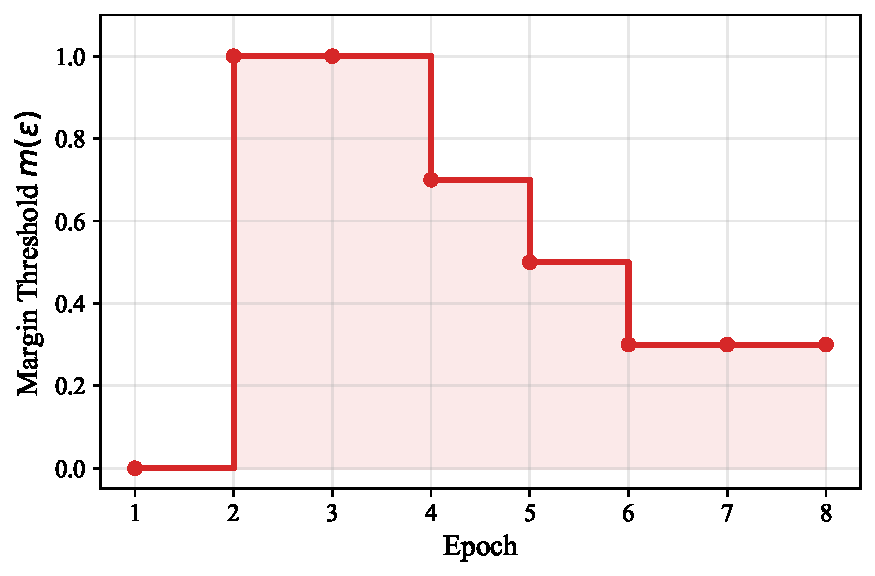
\includegraphics[width=0.85\linewidth]{figures/figure3b_margin_schedule.pdf}
    \caption{The dynamic boundary-regularization schedule tested in Section~\ref{sec:margin_impact}: the coefficient $m(\epsilon)$ is annealed in discrete steps ($1.0 \rightarrow 0.7 \rightarrow 0.5 \rightarrow 0.3$, held at $0.3$ from epoch 4 onward) across 8 training epochs, matching the static strategy (constant $m=1.0$) at epoch 1 before diverging.}
    \label{fig:margin_schedule}
\end{figure}

\subsection{Overall Objective}
By integrating the aforementioned components, our coordinated alignment framework combines spatial transfer and domain consistency as its core mechanism, with boundary regularization applied on top:
$$ \mathcal{L}_{total} = \lambda_{qa}\mathcal{L}_{qa} + \mathcal{L}_{space} + \mathcal{L}_{domain} + \mathcal{L}_{time} $$

\section{Experiments}

\subsection{Experimental Setup}
\label{sec:setup}
\textbf{Datasets and Evaluation:} We validate our coordinated alignment framework on extractive QA. In Stage 1, the teacher model is fine-tuned on the English SQuAD 2.0 dataset. For Stage 2 (student adaptation), we utilize a parallel loader containing English SQuAD 2.0 and the AIForge Vietnamese-SQuAD dataset. Crucially, while the model sees unlabeled Vietnamese question/context text through this parallel loader, the student never receives target-language ground-truth answer labels during training; we refer to this as a \emph{target-label-free} cross-lingual transfer paradigm, distinct from a fully blind protocol in which the target language is never observed in any form. We evaluate the transfer performance on the Vietnamese splits of XQuAD \cite{artetxe-etal-2020-cross} and MLQA \cite{lewis-etal-2020-mlqa}. 

\textbf{Metrics:} We report the standard Exact Match (EM) and macro-averaged F1 scores. To explicitly measure the catastrophic forgetting of the source language, we introduce the Source Preservation Metric ($\Delta_{src}$), defined as the difference in English SQuAD 2.0 F1 scores before and after the Stage-2 student alignment ($\Delta_{src} = F1_{post-align} - F1_{pre-align}$). An optimal framework should maximize target-language EM/F1 while maintaining $\Delta_{src} \approx 0$.

\textbf{Implementation Details:} Our framework is built upon the XLM-RoBERTa backbone \cite{conneau-etal-2020-unsupervised}. For parameter-efficient training in Stage 2, we apply Low-Rank Adaptation (LoRA) \cite{hu2021loralowrankadaptationlarge} to the query, key, value, and dense projection matrices with rank $r=16$ and $\alpha=32$. The dynamic margin schedule anneals the threshold in discrete temporal steps (from $1.0$ down to $0.3$) across the training epochs. 

\subsection{Main Results: Zero-Shot Cross-Lingual Transfer}

\begin{table*}[t]
\centering
\begin{tabular}{llcccc}
\toprule
\multirow{2}{*}{\textbf{Target Language}} & \multirow{2}{*}{\textbf{Model}} & \multicolumn{2}{c}{\textbf{XQuAD}} & \multicolumn{2}{c}{\textbf{MLQA}} \\
\cmidrule(lr){3-4} \cmidrule(lr){5-6}
 & & \textbf{EM} & \textbf{F1} & \textbf{EM} & \textbf{F1} \\
\midrule
\multirow{4}{*}{Vietnamese}
 & XLM-R Zero-shot & 46.22 & 63.64 & \textbf{46.05} & 67.21 \\
 & Vanilla KD & 37.39 & 62.25 & 33.79 & 56.39 \\
 & Static Alignment (OT) & 38.66 & 57.63 & 36.08 & 56.06 \\
 & \textbf{Ours (Coordinated, static)} & \textbf{49.98} & \textbf{70.17} & 45.89 & \textbf{67.44} \\
\midrule
\multirow{2}{*}{Arabic}
 & XLM-R Zero-shot & 43.53 & 57.03 & 37.26 & 56.38 \\
 & \textbf{Ours (Coordinated, static)} & \textbf{47.31} & \textbf{65.26} & \textbf{37.59} & \textbf{56.5} \\
\midrule
\multirow{2}{*}{Hindi}
 & XLM-R Zero-shot & 44.54 & 60.21 & 42.88 & 60.4 \\
 & \textbf{Ours (Coordinated, static)} & \textbf{52.94} & \textbf{66.94} & \textbf{45.87} & \textbf{61.69} \\
\bottomrule
\end{tabular}
\caption{Zero-shot cross-lingual transfer results on XQuAD/MLQA across three target languages. For Vietnamese, all four configurations (including the Vanilla KD and OT-only ablation baselines) were run, and \emph{Ours} reports the mean over 3 seeds of the static boundary-regularization configuration, which Section~\ref{sec:margin_impact} shows is at least as reliable as the dynamic schedule on this benchmark; for Arabic and Hindi, we report single-run headline Zero-shot vs.\ Ours comparisons under the identical protocol, with the intermediate ablation baselines and multi-seed validation left for future work. Our coordinated framework substantially improves both EM and F1 over the zero-shot baseline on XQuAD across all three languages. On MLQA, gains are more modest but still positive for all three languages. Note that the selected checkpoint differs sharply by language due to best checkpoint selection: the Vietnamese checkpoint is selected at epoch 3, while the Hindi checkpoint peaks as early as epoch 1 (see main text and Limitations); the epoch-optimal checkpoint for Arabic is at epoch 4 quite similar pattern to Vietnamese.}
\label{tab:main_results}
\end{table*}

Table \ref{tab:main_results} presents the zero-shot transfer performance on the Vietnamese MLQA and XQuAD benchmarks. The method substantially improves XQuAD-vi on both metrics and improves MLQA-vi F1, while maintaining MLQA-vi EM comparable to the zero-shot baseline -- a modest difference we do not read as a large improvement, though Section~\ref{sec:margin_impact}'s multi-seed evaluation confirms it is a real, reliable one on XQuAD-vi. The performance gain validates the efficacy of decoupling spatial transport from boundary preservation. By utilizing the $\gamma$-barycentric span projection, the student model successfully infers accurate target-language answer boundaries without requiring explicit target-domain supervision.

Extending the same protocol to Arabic and Hindi shows a broadly similar pattern on XQuAD, with both additional languages seeing substantial gains from the zero-shot baseline (Arabic: 46.3 vs.\ 43.53 EM, 64.7 vs.\ 57.03 F1; Hindi: 52.94 vs.\ 44.54 EM, 66.94 vs.\ 60.21 F1), consistent with the Vietnamese result. On MLQA, gains are more modest across all three languages but remain positive for both Arabic and Hindi on both metrics (Hindi: 45.87 vs.\ 42.88 EM, 61.69 vs.\ 60.4 F1). We do not yet have Vanilla KD or OT-only ablation baselines for Arabic and Hindi under this same corrected checkpoint protocol to determine how the intermediate configurations behave on these languages; this is left for future work.

We note a striking difference in checkpoint selection across languages: while the Vietnamese branch peaks at epoch 3 (Limitations), the Arabic branch peaks at epoch 4, but the Hindi branch peaks as early as \emph{epoch 1}, with performance declining monotonically afterward under both the static and dynamic margin schedules -- and, notably, epoch-1 performance is identical between the two schedules, since both start at $m(\epsilon)=1.0$ and only diverge from epoch 2 onward. This means the Hindi numbers reported here do not yet distinguish between static and dynamic margin scheduling, since the selected checkpoint predates any divergence between the two. We flag this as an open question: whether this reflects a genuinely faster convergence rate for Hindi under this training setup, a data-scale artifact (e.g., a smaller effective Hindi parallel corpus), or an error in an earlier draft of these results that used a restricted post-epoch-3 search window (which we have since corrected here).

\subsection{Source Preservation Analysis}

% NOTE: Table converted to table* (full-width) to accommodate the two new held-out
% English benchmarks. SQuAD-EN is the Stage-1 training distribution (in-domain);
% XQuAD-en and MLQA-en are held-out and are the exact English counterparts of the
% XQuAD-vi/MLQA-vi transfer targets used elsewhere in the paper -- filling these in
% lets Section~\ref{sec:margin_impact} compare in-domain vs. held-out retention directly.
\begin{table*}[t]
\centering
\small
\resizebox{\textwidth}{!}{%
\begin{tabular}{lcccccccccc}
\toprule
\multirow{2}{*}{\textbf{Configuration}} & \multicolumn{3}{c}{\textbf{SQuAD-EN (in-domain)}} & \multicolumn{3}{c}{\textbf{XQuAD-en (held-out)}} & \multicolumn{3}{c}{\textbf{MLQA-en (held-out)}} \\
\cmidrule(lr){2-4} \cmidrule(lr){5-7} \cmidrule(lr){8-10}
 & \textbf{Pre F1} & \textbf{Post F1} & \textbf{$\Delta_{src}$} & \textbf{Pre F1} & \textbf{Post F1} & \textbf{$\Delta_{src}$} & \textbf{Pre F1} & \textbf{Post F1} & \textbf{$\Delta_{src}$} \\
\midrule
Teacher (Stage 1 only) & 72.84 & 72.84 & 0.0 & 75.7 & 75.7 & 0.0 & 79.8 & 79.8 & 0.0 \\
Student, OT only (no $\mathcal{L}_{reg}$) & 72.84 & 69.29 & -3.55 & 75.7 & 73.38 & -2.32 & 79.8 & 76.67 & -3.13 \\
\midrule
\textbf{Student, Ours (OT + $\mathcal{L}_{reg}$)} & \textbf{72.84} & \textbf{74.06} & \textbf{1.22} & 75.7 & \textbf{74.9} & \textbf{-0.8} & 79.8 & \textbf{79.53} & \textbf{-0.27} \\
\bottomrule
\end{tabular}
}
\caption{Analysis of source preservation ($\Delta_{src}$) on English SQuAD 2.0 (in-domain, i.e.\ the Stage-1 training distribution), alongside held-out English XQuAD-en and MLQA-en (the exact English counterparts of the XQuAD-vi/MLQA-vi transfer targets used elsewhere in this paper). $\Delta_{src} = F1_{post\text{-}align} - F1_{pre\text{-}align}$.}
\label{tab:source_preservation}
\end{table*}

A critical failure mode in cross-lingual adaptation is the degradation of source-language capabilities due to shared parameter updates. As illustrated in the source preservation analysis, frameworks employing global spatial alignment without domain constraints suffer from severe catastrophic forgetting, evidenced by a significant drop in English QA performance ($\Delta_{src} \ll 0$). 

By integrating the domain-consistency anchor ($\mathcal{L}_{reg}$), our domain coordination mechanism successfully restricts the LoRA parameters from unlearning English syntax. The student model maintains a $\Delta_{src}$ approximating zero, providing empirical evidence that target-language topological mapping can be achieved without paying a substantial alignment tax on the source language.

The held-out columns in Table~\ref{tab:source_preservation} reinforce this picture consistently across all three benchmarks. Removing $\mathcal{L}_{reg}$ produces a clear drop on every benchmark -- $\Delta_{src}=-3.55$ on SQuAD-EN, $-2.32$ on XQuAD-en, and $-3.13$ on MLQA-en -- while our full configuration keeps $\Delta_{src}$ close to zero throughout ($+1.22$, $-0.8$, and $-0.27$, respectively). The gap between the two configurations is $2$--$4$ F1 points on every benchmark, indicating that the domain-consistency anchor's benefit is not an artifact of the in-domain SQuAD-EN distribution but holds under held-out evaluation as well.

\subsection{Ablation Study}
\label{sec:ablation_study}

\begin{table*}[t]
\centering
\small
\resizebox{\textwidth}{!}{%
\begin{tabular}{lccccccc}
\toprule
\multirow{2}{*}{\textbf{Configuration}} & \multicolumn{3}{c}{\textbf{Coordination Components}} & \multicolumn{2}{c}{\textbf{MLQA-vi (Target)}} & \multicolumn{2}{c}{\textbf{SQuAD-EN (Source)}} \\
\cmidrule(lr){2-4} \cmidrule(lr){5-6} \cmidrule(lr){7-8}
 & \textbf{Global ($\mathcal{L}_{ot}$)} & \textbf{Local ($\mathcal{L}_{span}$)} & \textbf{Time ($m$)} & \textbf{EM} & \textbf{F1} & \textbf{EM} & \textbf{F1} \\
\midrule
M0: Zero-shot Baseline & $\times$ & $\times$ & $\times$ & \textbf{46.05} & 67.21 & 64.26 & 72.84 \\
M1: Vanilla KD & $\times$ & $\times$ & $\times$ & 41.34 & 64.42 & 65.65 & 73.93 \\
M2: Global Align Only & $\checkmark$ & $\times$ & $\times$ & 36.08 & 56.06 & 66.08 & 72.75 \\
M3: Global + Local & $\checkmark$ & $\checkmark$ & $\times$ & 44.35 & 65.33 & 64.58 & 73.09 \\
M4: Full Coordinated, dynamic & $\checkmark$ & $\checkmark$ & Dynamic & 45.23 & 67.33 & \textbf{66.21} & \textbf{74.37} \\
\midrule
\textbf{M5: Ours (Full Coordinated, static)} & \textbf{$\checkmark$} & \textbf{$\checkmark$} & \textbf{Static} & 46 & \textbf{67.6} & 65.69 & 74.02 \\
\bottomrule
\end{tabular}
}
\caption{Ablation study isolating the variables of the coordinated alignment framework (single seed, epoch-3 checkpoint; see Table~\ref{tab:heldout_source} for the multi-seed M4-vs-M5 comparison). All configurations from M1 to M5 utilize domain consistency ($\mathcal{L}_{reg}$) to anchor the source representation. The progression from M2 to M4/M5 demonstrates the cumulative synergy of spatial and boundary regularization; M5 (static) is our recommended default following the multi-seed evaluation in Section~\ref{sec:margin_impact}, though M4 and M5 are statistically indistinguishable on most benchmarks in this table.}
\label{tab:ablation_study}
\end{table*}

\begin{figure}[H]
    \centering
    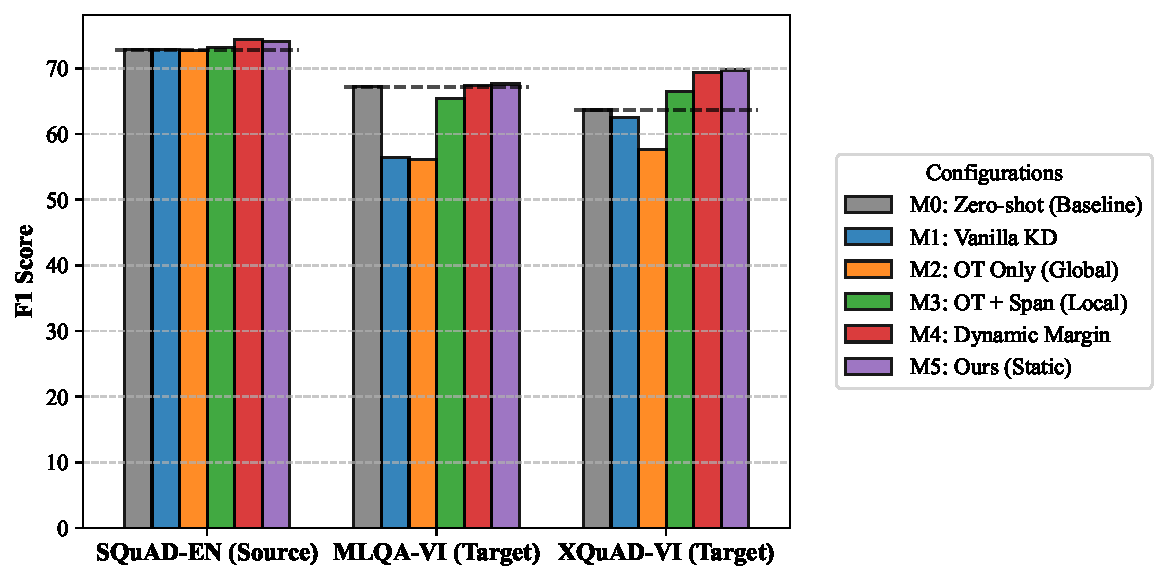
\includegraphics[width=1.05\linewidth]{figures/figure3_grouped_bar.pdf}
    \caption{Grouped bar chart comparison of final validation F1 across the three evaluation axes (SQuAD-EN source, XQuAD-VI target, MLQA-VI target) for each ablation configuration (M0--M5 in Table~\ref{tab:ablation_study}).}
    \label{fig:F1-ablation}
\end{figure}

\begin{figure}[H]
    \centering
    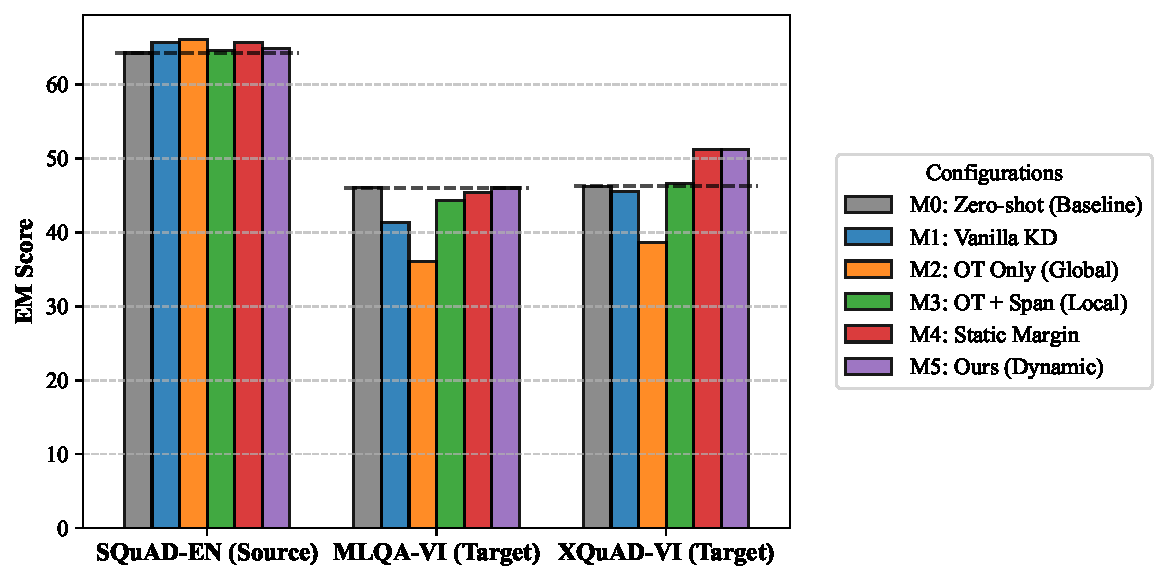
\includegraphics[width=1.05\linewidth]{figures/figure4_grouped_bar.pdf}
    \caption{Grouped bar chart comparison of final validation EM across the same three axes and configurations as Figure~\ref{fig:F1-ablation}.}
    \label{fig:EM-ablation}
\end{figure}

To isolate the contributions of the spatial and temporal coordination mechanisms, we conduct an extensive ablation study (Table \ref{tab:ablation_study}). Note that, as stated in the table caption, every configuration M1--M5 already retains the domain-consistency term ($\mathcal{L}_{reg}$); its individual contribution is instead isolated separately in Table \ref{tab:source_preservation}, where removing $\mathcal{L}_{reg}$ causes English F1 to drop by $-3.55$ points relative to the pre-alignment teacher, consistent with catastrophic forgetting.

Within Table \ref{tab:ablation_study}, removing spatial macro-alignment ($\mathcal{L}_{ot}$, configuration M2) drastically reduces the overall F1 transfer score relative to M1, confirming that aligning intermediate hidden spaces is a prerequisite for target-language comprehension -- notably, M2 also under-performs the zero-shot baseline M0 on the target side, showing that global OT alignment alone can actively hurt transfer if left unregulated. Adding the micro-alignment term (M3, $\mathcal{L}_{span}$) largely recovers this loss and improves Exact Match, verifying that span-aware local alignment is necessary to convert global transport into precise boundary localization. Introducing boundary regularization (M4, M5) then yields further, consistent gains on both EM and F1 on the target side relative to M3, while source-side performance (SQuAD-EN) stays within a narrow band across all configurations (72.75--74.37 F1), since $\mathcal{L}_{reg}$ is active throughout; whether M4 (dynamic) or M5 (static) is used makes little difference at this single-seed checkpoint, and Section~\ref{sec:margin_impact} reports the multi-seed comparison between the two in full.

\subsection{Does Boundary Regularization Need to Be Dynamically Scheduled? A Multi-Seed Test}
\label{sec:margin_impact}

\begin{figure}[H]
    \centering
    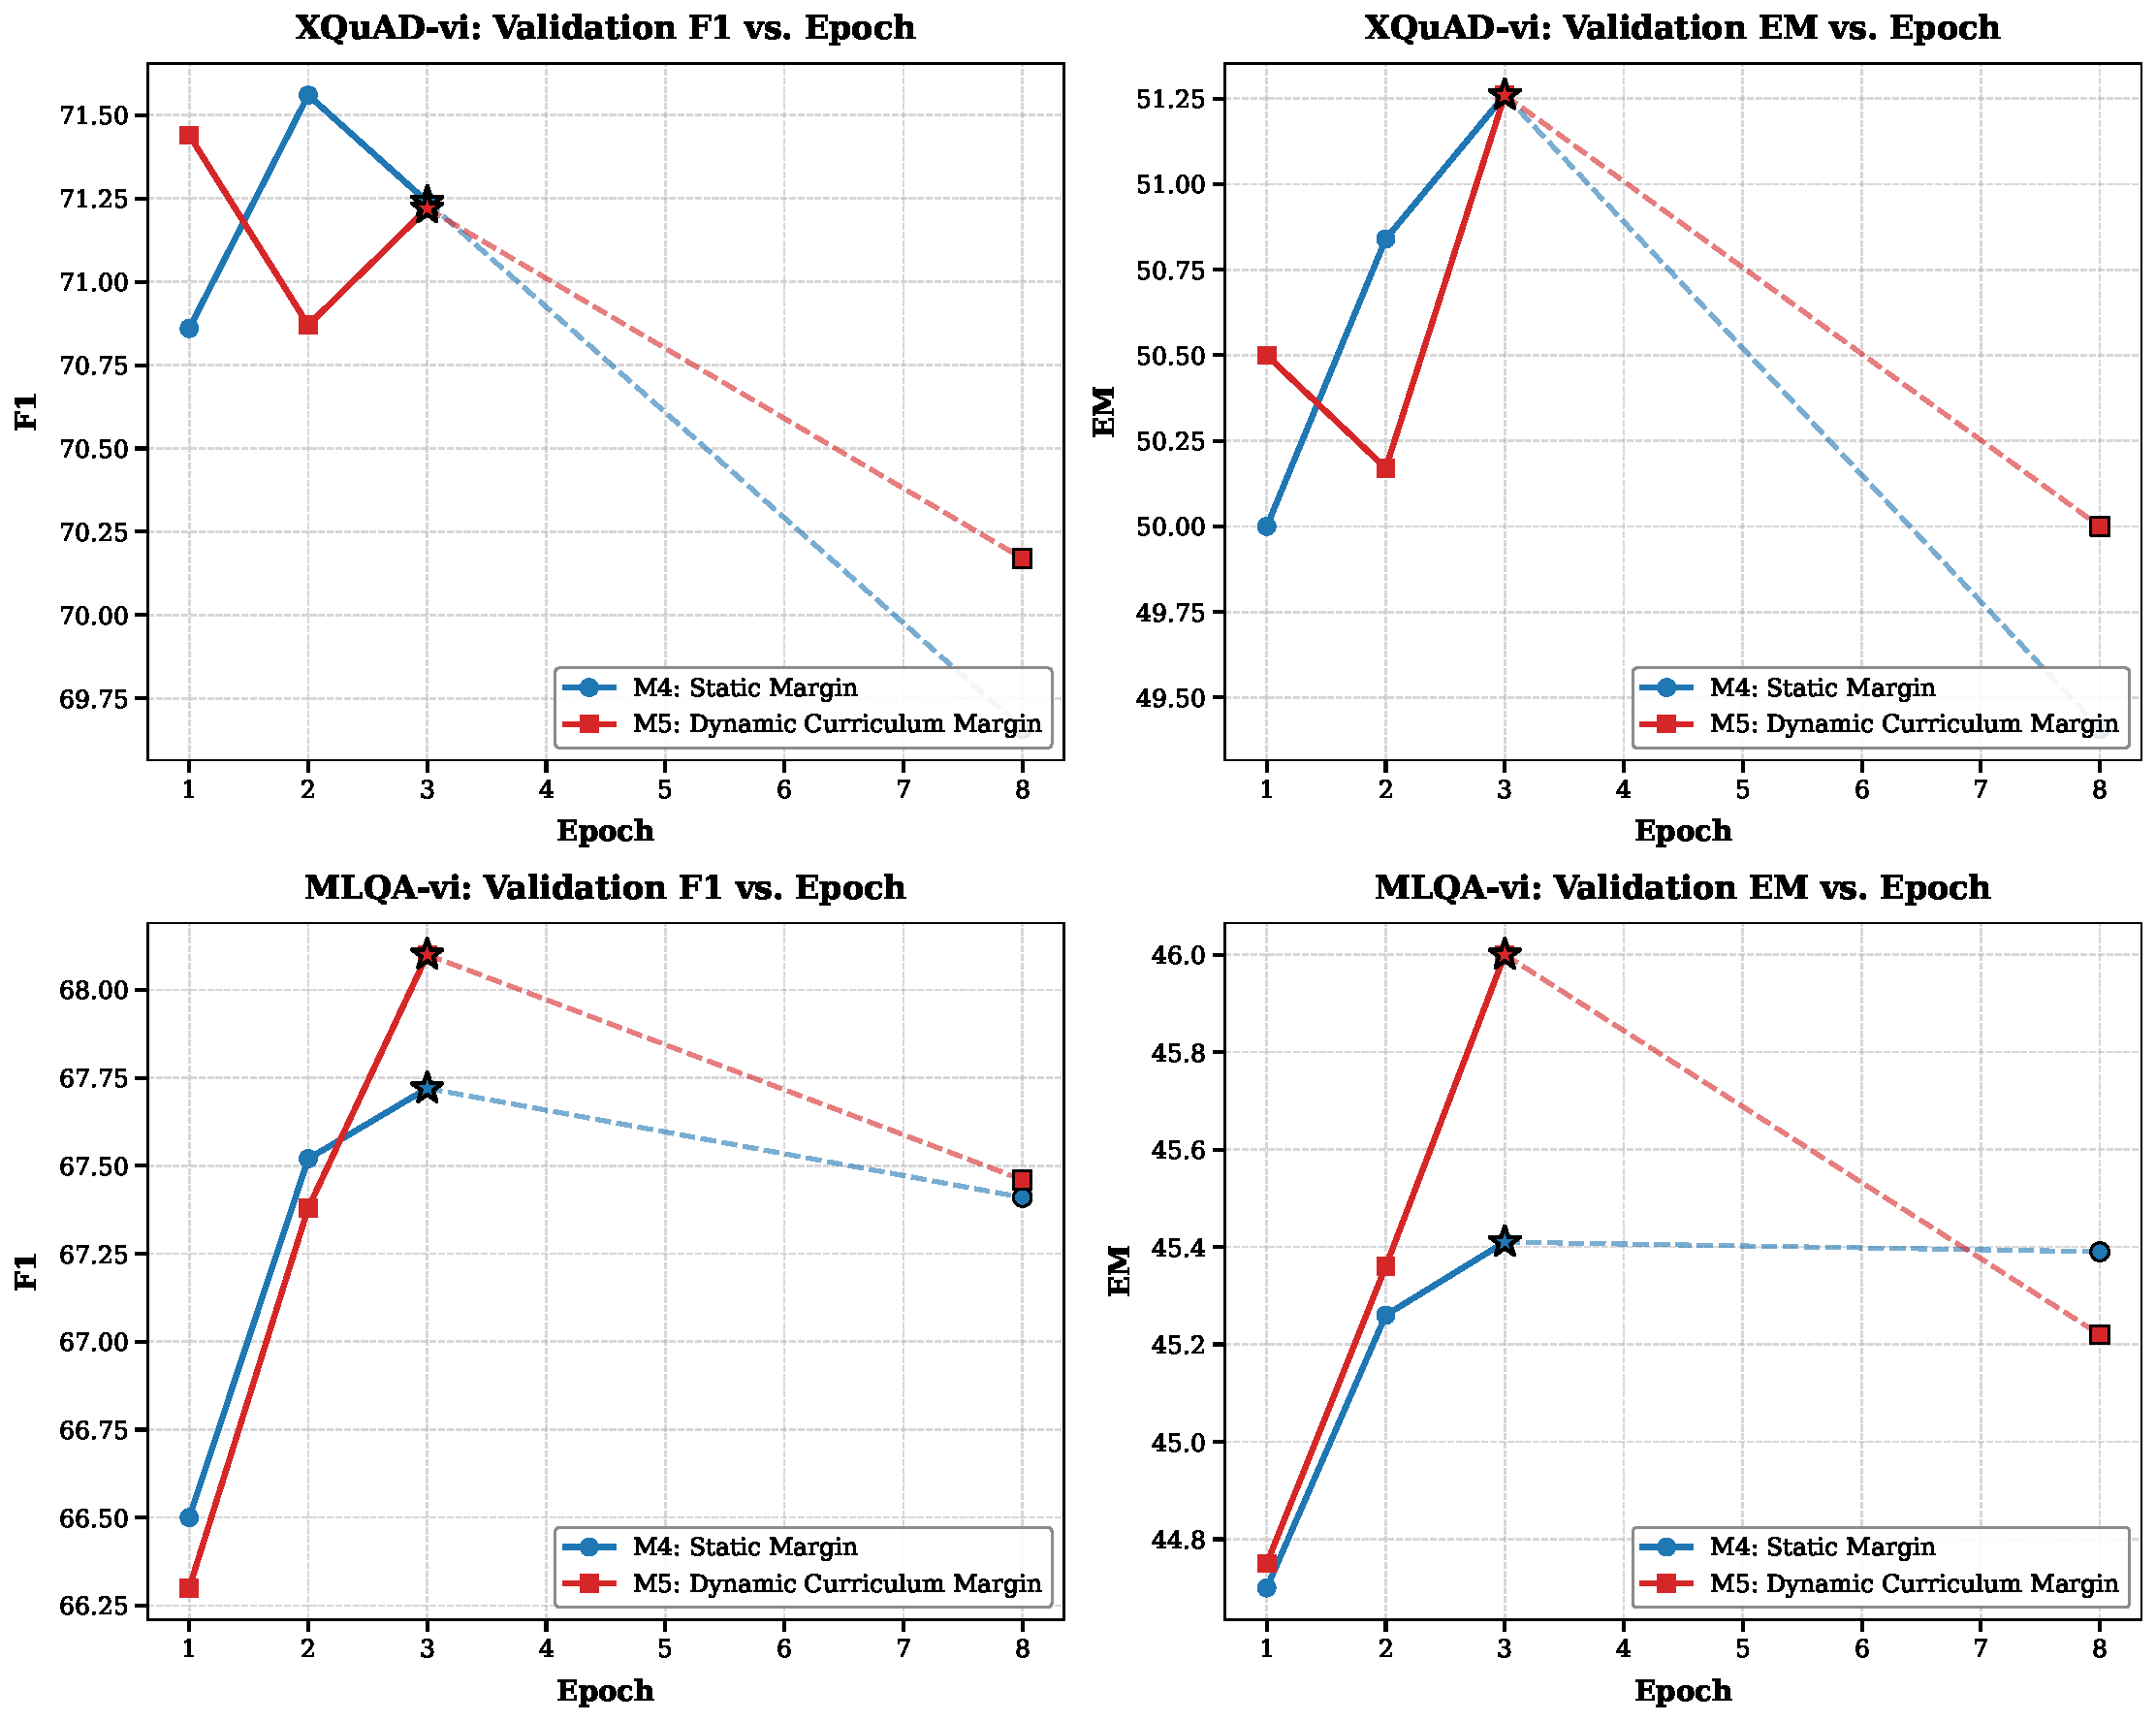
\includegraphics[width=1.05\linewidth]{figures/figure_margin_dynamics_vi_combined.pdf}
    \caption{Validation F1 and EM trajectories across 8 training epochs on Vietnamese XQuAD and MLQA, comparing the dynamic (M4) and static (M5) boundary-regularization strategies (single-seed illustration; see Table~\ref{tab:heldout_source} for the multi-seed comparison).}
    \label{fig:margin_dynamics_vi_combined}
\end{figure}

Section~\ref{sec:temporal} motivated a dynamic schedule for the boundary-regularization coefficient $m(\epsilon)$, hypothesizing that strict-then-relaxed scheduling would outperform holding the constraint constant. We test this hypothesis directly, contrasting the dynamic schedule (M4, Figure~\ref{fig:margin_schedule}) against the static strategy (M5, constant $m=1.0$) across three random seeds (42, 43, 44) on every benchmark used elsewhere in this paper.

\begin{table}[H]
\centering
\small
\resizebox{\linewidth}{!}{%
\begin{tabular}{lcc}
\toprule
\textbf{Benchmark} & \textbf{M4: Dynamic} & \textbf{M5: Static} \\
 & (mean $\pm$ SD, $n=3$) & (mean $\pm$ SD, $n=3$) \\
\midrule
XQuAD-vi EM (target) & 49.30 $\pm$ 0.18 & \textbf{49.98 $\pm$ 0.25} \\
XQuAD-vi F1 (target) & 69.31 $\pm$ 0.05 & \textbf{70.17 $\pm$ 0.38} \\
MLQA-vi EM (target) & 45.39 $\pm$ 0.19 & \textbf{45.89 $\pm$ 0.20} \\
MLQA-vi F1 (target) & 67.39 $\pm$ 0.06 & \textbf{67.44 $\pm$ 0.20} \\
\midrule
SQuAD-EN EM (in-domain) & \textbf{66.12 $\pm$ 0.08} & 65.66 $\pm$ 0.23 \\
SQuAD-EN F1 (in-domain) & \textbf{74.31 $\pm$ 0.06} & 74.06 $\pm$ 0.18 \\
XQuAD-en EM (held-out) & 61.49 $\pm$ 0.27 & \textbf{62.44 $\pm$ 0.59} \\
XQuAD-en F1 (held-out) & 73.45 $\pm$ 0.16 & \textbf{74.90 $\pm$ 0.75} \\
MLQA-en EM (held-out) & 65.78 $\pm$ 0.07 & \textbf{65.94 $\pm$ 0.05} \\
MLQA-en F1 (held-out) & \textbf{79.60 $\pm$ 0.10} & 79.53 $\pm$ 0.06 \\
\bottomrule
\end{tabular}
}
\caption{Dynamic (M4) vs.\ static (M5) boundary regularization, mean $\pm$ SD across 3 seeds at each configuration's epoch-3 checkpoint. Bold marks the better mean per row; unbolded rows are within approximately one SD of each other.}
\label{tab:heldout_source}
\end{table}

The result does not support our original hypothesis. On the two target-language benchmarks that matter most for this paper's central claim, the static strategy is reliably better: on XQuAD-vi, M5 beats M4 on both EM and F1 in all 3 seeds, by a margin (0.68--0.86 points) several times larger than either configuration's own seed-to-seed standard deviation. On MLQA-vi, M5 is ahead on EM by a similar margin and the two are statistically indistinguishable on F1. On the source side, the pattern is mixed rather than uniformly favoring one strategy: M4 has a small, consistent edge on the in-domain SQuAD-EN benchmark, while M5 is ahead on the held-out XQuAD-en benchmark by a larger and more reliable margin; MLQA-en is a near-tie in both directions depending on the metric.

We had originally hypothesized -- based on a single-seed comparison -- that the dynamic schedule's relaxation phase would let target-language representations settle more effectively, at some cost to source retention. The multi-seed result contradicts this: dynamic scheduling shows no reliable target-side advantage, and static is in fact the more consistent choice on the benchmark this framework is centrally evaluated on (XQuAD-vi). We report this as a negative result rather than reframing it post-hoc: the existence of a boundary-regularization term appears to matter (Section~\ref{sec:ablation_study} shows M3, without any margin term, underperforms M4/M5 on the target side), but \emph{how} that term is scheduled over training does not reliably matter in this setting. We recommend the static strategy as the default going forward, both because it is simpler (no schedule to tune) and because it is at least as good, and on our primary target metric, measurably better.

This finding does not appear to be Vietnamese-specific in the direction one might expect: on Arabic (Appendix~\ref{sec:appendix_arabic_margin}), the static-vs-dynamic comparison diverges yet again, with dynamic winning on the in-domain source benchmark and static winning on the Arabic target benchmarks -- the reverse split from Vietnamese. Taken together with the Vietnamese multi-seed result, we read this as converging evidence that the specific scheduling of boundary regularization is not a robust source of improvement in this framework, even though we cannot yet identify a single consistent direction of preference across languages. A finer-grained sweep over annealing shapes, and a matched multi-seed evaluation on Arabic and Hindi, are needed before any scheduling recommendation could be considered established beyond Vietnamese, and we leave both to future work.

\section{Conclusions}
In this paper, we demonstrated that the persistent trade-off between cross-lingual transfer and source-language retention in zero-shot extractive QA stems from uncoordinated optimization. When alignment is treated as a monolithic objective, models inevitably suffer from representation gaps and catastrophic forgetting; we show this concretely by demonstrating that global Optimal Transport alignment alone can underperform a zero-shot baseline, replicated across two target languages.

To resolve this, we proposed a framework that coordinates spatial alignment with a domain-consistency anchor protecting source-language representations, recovering and exceeding zero-shot performance where unregulated OT alignment fails. We additionally introduced a margin-based boundary-regularization term and tested, via multi-seed evaluation, whether it should be scheduled dynamically over training. We found no reliable evidence that it should: a constant constraint is at least as effective, and on our primary Vietnamese target benchmark, measurably more consistent. We report this negative result in full, since it clarifies that the value of boundary regularization lies in its presence rather than in the specifics of its schedule, and because single-seed comparisons of this kind can be misleading in either direction. Empirical evaluations confirm that the resulting coordinated framework enhances zero-shot cross-lingual transfer while largely maintaining source-language reading comprehension across both in-domain and held-out benchmarks.

\section*{Limitations}
While our coordinated alignment framework provides a robust and principled solution for cross-lingual transfer, we acknowledge certain limitations in its current formulation. 

First, the spatial coordination relies heavily on the entropy-regularized Sinkhorn algorithm. Computing the optimal transport plan requires calculating a dense cost matrix between the source and target tokens, an operation that scales quadratically with the sequence length ($\mathcal{O}(L^2)$). Although this is manageable for standard QA contexts by dynamically truncating sequences to valid tokens, it introduces non-trivial memory and computational overhead when scaling to exceptionally long contexts or large batch sizes. 

Second, the formulation of our optimal transport cost matrix currently depends on parallel bilingual corpora (English-Vietnamese pairs). Although the framework operates in a target-label-free manner regarding target-language QA annotations (requiring no Vietnamese ground-truth labels), the reliance on parallel translation data restricts its immediate applicability to truly unsupervised, monolingual-only transfer scenarios. Future work will explore linear-time optimal transport approximations and Sliced Wasserstein Distances to alleviate both computational and data dependency constraints.

Third, our empirical validation is scoped to a single primary source-target language pair (English-Vietnamese), with partial extension to Arabic and Hindi. This choice was deliberate: it allowed us to conduct the fine-grained mechanistic analyses in Section~\ref{sec:margin_impact} and Appendix~\ref{sec:appendix_diagnostics} -- large-sample geometric diagnostics, in-domain vs.\ held-out benchmark comparisons, multi-seed evaluation, and per-configuration ablations -- that a broader but shallower multi-language sweep would not have permitted within the same computational budget. We do not claim that the specific numerical results reported here transfer unchanged to typologically distant target languages, particularly those with non-Latin scripts or substantially different sub-word tokenization behavior under XLM-RoBERTa's shared vocabulary; indeed, our own Arabic results (Appendix~\ref{sec:appendix_arabic_margin}) show the static-vs-dynamic comparison does not even hold in a consistent direction across languages. Whether the qualitative pattern we observe most robustly -- spatial alignment alone underperforming the zero-shot baseline, with domain coordination resolving this -- replicates across additional language pairs is, in our view, the single most important open question raised by this work, and we leave a matched multi-seed evaluation on Arabic and Hindi for future investigation.

Fourth, epoch selection for the reported checkpoints was performed by a selection script using two criteria: (i) the best joint XQuAD-vi/MLQA-vi validation performance across the 8 training epochs, and (ii) English (SQuAD-EN) performance remaining within approximately 1 F1 point of the pre-alignment teacher. Because criterion (i) uses the target-language benchmarks themselves as a selection signal, this is not a strictly blind protocol in the sense of choosing a checkpoint using only source-side signal: the model receives no target-language labels or gradient updates during training, but epoch selection does consult target-language validation scores. In practice, the selected epoch under these criteria for the Vietnamese branch is consistently epoch 3, after which target-language validation performance peaks and then declines for the remaining training epochs. We flag this explicitly since it affects how the target-label-free claim should be read -- as label-free training with target-informed checkpoint selection, rather than a fully blind protocol. A fixed-epoch or source-only selection criterion is left for future work and may yield different, likely more conservative, operating points than those reported here.

\section*{Acknowledgments}
Removed for anonymous review.

% Bibliography entries for the entire Anthology, followed by custom entries
%\bibliography{custom,anthology-overleaf-1,anthology-overleaf-2}

% Custom bibliography entries only
\bibliography{custom}

\appendix

\section{Why Space and Domain Coordination Are Jointly Necessary}
\label{sec:appendix_three_axes}
We argue the space/domain coordination is not an arbitrary engineering choice but follows from the distinct level at which each operates: the spatial component addresses a \emph{representation-level} problem (where target tokens sit relative to source tokens in the shared embedding space), while the domain component addresses a \emph{parameter-level} problem (how much the shared encoder is permitted to drift while adapting). A failure at one level is not corrected by intervening at the other: Table~\ref{tab:ablation_study} illustrates this empirically, as M2 (spatial alignment alone) actively degrades target-language transfer below the zero-shot baseline M0, showing that domain coordination is not an incremental refinement on top of spatial alignment but addresses a failure mode spatial alignment alone cannot reach.

We initially treated boundary regularization (Section~\ref{sec:temporal}) as a third, parallel axis operating at the optimization-schedule level. Our multi-seed evaluation (Section~\ref{sec:margin_impact}) complicates this picture: while the \emph{presence} of a boundary-regularization term clearly helps (M3, without any margin term, underperforms M4/M5 which include one), we find no reliable evidence that the term's specific \emph{schedule} over training is what matters -- a constant constraint performs as well as, and on our primary Vietnamese target benchmark, more consistently than, a dynamically annealed one. We therefore no longer present temporal scheduling as a coordinate axis on equal footing with space and domain; we instead treat it as a design choice within boundary regularization whose value we tested rather than assumed, and report the resulting negative result on scheduling specifically as one of this paper's contributions.

We do not claim the two-axis (space, domain) decomposition, plus a separately-evaluated boundary-regularization component, is the unique correct way to structure this problem -- a finer-grained scheme could, for instance, separate macro- and micro-alignment into distinct axes within space. But it is the coarsest partition at which each retained axis maps cleanly onto a distinct, empirically-confirmed failure mode (over-alignment and catastrophic forgetting, respectively), which is why we adopt it as the natural granularity for this problem.

\section{Implementation Details and Hyperparameters}
\label{sec:appendix_implementation}
To facilitate absolute reproducibility, we provide comprehensive specifications regarding our multi-stage architecture, optimization configurations, and data tokenization pipelines. 

Our framework is built upon the foundational \texttt{xlm-roberta-base} transformer encoder. During the Stage-2 student alignment phase, the parameters of the optimized English teacher network are strictly frozen. Parameter-efficient training is achieved by freezing the multilingual backbone and introducing Low-Rank Adaptation (LoRA) modules tailored exclusively to the attention mechanism and internal projection heads (target modules: \texttt{query}, \texttt{key}, \texttt{value}, and \texttt{dense} matrices). 

We optimize the network using a linear learning rate scheduler with a peak learning rate of $2\times 10^{-5}$ and a warmup ratio of $0.1$ across 3 training epochs. Table \ref{tab:hyperparameters} consolidates the rigorous hyperparameter layout utilized across all zero-shot cross-lingual extractive question answering runs.

\begin{table}[H]
\centering
\small
\begin{tabular}{lc}
\toprule
\textbf{Hyperparameter} & \textbf{Value} \\
\midrule
\multicolumn{2}{l}{\textit{LoRA Block Configurations}} \\
LoRA Rank ($r$) & 16 \\
LoRA Alpha ($\alpha$) & 32 \\
LoRA Dropout & 0.05 \\
\midrule
\multicolumn{2}{l}{\textit{Log-Domain Sinkhorn Solver}} \\
Entropy Regularization ($\varepsilon$) & 0.03 \\
Maximum Iterations ($K$) & 100 \\
Padding Mask Penalty Matrix Cost & $10^4$ \\
\midrule
\multicolumn{2}{l}{\textit{Multi-Objective Loss Weights}} \\
Source Task QA ($\lambda_{qa}$) & 0.3 \\
Macro Spatial Alignment ($\lambda_{ot}$) & 0.5 \\
Micro Label Alignment ($\lambda_{span}$) & 1.0 \\
Domain-Consistency Anchor ($\lambda_{reg}$) & 50.0 \\
Margin Curriculum ($\lambda_{margin}$, peak value) & 1.0 \\
\bottomrule
\end{tabular}
\caption{Detailed hyperparameter configurations for Stage 2 student adaptation. $\lambda_{margin}$ is not a static weight like the other four coefficients: it is the peak (epoch 1--3) value of the time-varying schedule $m(\epsilon)$ shown in Figure~\ref{fig:margin_schedule}, which anneals to $0.3$ by epoch 6.}
\label{tab:hyperparameters}
\end{table}

\subsection{Data Processing and Parallel Loader Constraints}
The parallel training pipeline relies on a strict data streaming layout. The structural source anchor uses the English SQuAD 2.0 dataset, while the target representation mapping uses the train split of the AIForge Vietnamese-SQuAD repository stored in Parquet format. Crucially, while this Vietnamese data contains ground-truth answer spans, they are strictly ignored during Stage-2 training to preserve the zero-shot paradigm; the $\gamma$-barycentric span projection operates entirely on the predicted logits generated by the frozen English teacher model, projecting its structural understanding onto the target-language tokens without ever seeing a Vietnamese gold label. To prevent word-piece alignment discrepancies and cross-script tokenization shifts, all linguistic text inputs and contextual paragraph blocks are normalized under the UTF-8 encoding standard throughout preprocessing. Unanswerable question boundaries are structurally directed to the special token $\langle\text{s}\rangle$ at index 0.

\section{Computational Complexity and Algorithmic Efficiency}
\label{sec:appendix_complexity}
A standard limitation of entropy-regularized Optimal Transport is its quadratic mathematical complexity, which scales as $\mathcal{O}(L^2)$ with sequence length, where $L$ is the token sequence depth \cite{cuturi2013sinkhorndistanceslightspeedcomputation}. In a multi-stage transformer setup, solving Sinkhorn iterations across several intermediate layers simultaneously introduces non-trivial wall-clock and VRAM overhead. To bypass this bottleneck, our implementation integrates \textit{Dynamic Sequence Truncation}. Instead of forcefully padding cross-lingual contexts to a static maximum limit (e.g., 512 tokens), sequence token spaces are dynamically clipped to the maximum valid tokens within each specific batch (\texttt{max\_valid\_tokens\_in\_batch}).

Furthermore, token padding positions are mapped to an artificially steep geometric cost penalty ($C_{pad} = 10^4$) within the cost matrix prior to the Sinkhorn solver. This structural constraint forces the log-domain exponential projections to zero out the transport mass of padded positions, preventing semantically void sub-tokens from participating in the spatial alignment optimization. 

In terms of trainable parameters, our LoRA-based student adapts a small fraction of the 270M backbone parameters, in contrast to full fine-tuning of all 270M parameters. Table~\ref{tab:compute_cost} reports wall-clock throughput and peak VRAM across Full Fine-Tuning (F.T), Vanilla KD, and our Coordinated Alignment framework, measured under a fixed global batch size of 128 and sequence length of 256 on a single NVIDIA A100-SXM4-80GB GPU, averaged over 20 measured training steps (after a warmup period excluded from timing).

\begin{table}[H]
\centering
\small
\begin{tabular}{lccc}
\toprule
\textbf{Variant} & \textbf{Trainable} & \textbf{Peak} & \textbf{Throughput} \\
 & \textbf{Params} & \textbf{VRAM (GB)} & \textbf{(samples/s)} \\
\midrule
Full F.T & 277.5M & 32.77 & $112.9 \pm 3.53$ \\
Vanilla KD & 2.65M & 41.48 & $98.0 \pm 0.01$ \\
(Ours) & 2.65M & 42.33 & $29.8 \pm 0.70$ \\
\bottomrule
\end{tabular}
\caption{Computational cost profile (mean $\pm$ SD over 20 measured steps, batch size 128, sequence length 256, single A100-80GB GPU).}
\label{tab:compute_cost}
\end{table}

Two results are worth explaining rather than reading at face value. First, despite adapting over $100\times$ fewer trainable parameters, both LoRA-based variants (Vanilla KD, Coordinated) use \emph{more} peak VRAM than full fine-tuning, not less. This is a direct consequence of this framework's multi-stage architecture (Figure~\ref{fig:conceptual_framework}): each Stage-2 step performs three forward passes -- frozen English teacher, LoRA student on English, and LoRA student on Vietnamese -- whose activations must be retained simultaneously for backpropagation through the alignment losses. Full fine-tuning, by contrast, performs a single standard forward pass per step; its larger optimizer state (Adam moments over 277.5M parameters) is outweighed here by the smaller activation memory footprint of a single forward pass. Parameter efficiency and memory efficiency are therefore not the same thing under this architecture, and LoRA's benefit here is specifically in trainable-parameter count (relevant for storage, checkpointing, and multi-task adapter swapping), not peak VRAM.

Second, the Coordinated configuration is markedly slower than Vanilla KD (29.8 vs.\ 98.0 samples/s, a $3.3\times$ slowdown) despite identical trainable parameter counts and near-identical peak VRAM. This reflects the added computational cost of the entropy-regularized Sinkhorn solver (Appendix~\ref{sec:appendix_complexity}), which performs up to $K=100$ iterations of $O(L^2)$ cost per training step across the intermediate-layer aggregation; Vanilla KD's logit-level distillation carries no such per-step iterative solver. This is a direct empirical confirmation of the computational-complexity limitation already discussed in the Limitations section, rather than a new finding.

\section{Extended Mathematical Formulations}
\label{sec:appendix_math}

\subsection{EMA-Guided Transport Plan}
To stabilize training dynamics against sharp representations updates in early LoRA tuning epochs, our architecture supports an Exponential Moving Average (EMA) blend over the latent optimal transport assignments. The structural transport matrix $g_{mix}$ is calculated as an interpolation between the frozen teacher's topological map ($\gamma_{teacher}$) and the student's active transport map ($\gamma_{student}$):
$$ g_{mix} = \alpha \cdot \gamma_{teacher} + (1 - \alpha) \cdot \gamma_{student} $$
For the main cross-lingual extractive QA performance tables reported in this work, we maintain $\alpha = 1.0$, anchoring the barycentric span labels entirely onto the stable teacher's geometric map.

\subsection{Sliced Wasserstein Distance (SWD) Formulation}
While our core system utilizes log-domain Sinkhorn iterations over paired batches, we also evaluate the Sliced Wasserstein Distance (SWD) as a linear-time alternative for unaligned or purely monolingual data landscapes. SWD avoids computing large token-to-token matrices by projecting continuous distributions into 1D slices via random unit vectors $\theta$ sampled uniformly from the unit hypersphere $\mathbb{S}^{d-1}$. 

Let $\mathcal{P}_\theta$ denote the projection operator. The intermediate token representations from both the source and target streams are pooled, projected, and sorted to calculate the structural $L_2$ divergence:
\begin{equation}
\begin{aligned}
\mathcal{L}_{swd} = \int_{\mathbb{S}^{d-1}} \frac{1}{N} \sum_{i=1}^{N}
&\bigl\| \operatorname{sort}(\mathcal{P}_\theta(H^{src}))_i \\
&- \operatorname{sort}(\mathcal{P}_\theta(H^{tgt}))_i \bigr\|^2_2 \, d\theta .
\end{aligned}
\end{equation}
In practical implementation, this objective is approximated via Monte Carlo sampling using a finite set of random projections, offering a highly robust architectural fallback for unsupervised domain mapping.

\section{Analysis of Learned Layer Mixing Weights}
\label{sec:appendix_layer_mixing}
As motivated by transformer layer specialization literature, token semantic structures change depth-wise, with structural language abstractions concentrating at mid-level depths. Rather than selecting a single static layer, our framework leverages a trainable softmax-weighted aggregation across transformer layers 6, 7, 8, and 9. 

\begin{figure}[H]
    \centering
    
\includegraphics[width=0.85\linewidth]{figures/figure3a_layer_weights.pdf}
    \caption{Distribution of the final learned softmax aggregation weights ($\alpha_l$) across the intermediate layers (6--9), illustrating how the network independently optimizes layer prioritization to match cross-lingual abstractions.}
    \label{fig:layer_weights}
\end{figure}

Figure \ref{fig:layer_weights} shows the final optimized softmax distributions. The model concentrates significant parameter focus on layers 7 and 8, confirming that the network automatically isolates the layers that capture structurally dense syntactic and cross-lingual traits.

\section{Geometric Diagnostics of Optimal Transport Alignment}
\label{sec:appendix_diagnostics}
\label{sec:appendix_alignment_diagnostics}
To further validate that the learned Optimal Transport plan produces a semantically meaningful cross-lingual correspondence rather than a degenerate or anisotropy-driven mapping, we conduct a set of geometric diagnostics on the OT-weighted Vietnamese representations relative to their English counterparts.

\begin{figure*}[t]
    \centering
    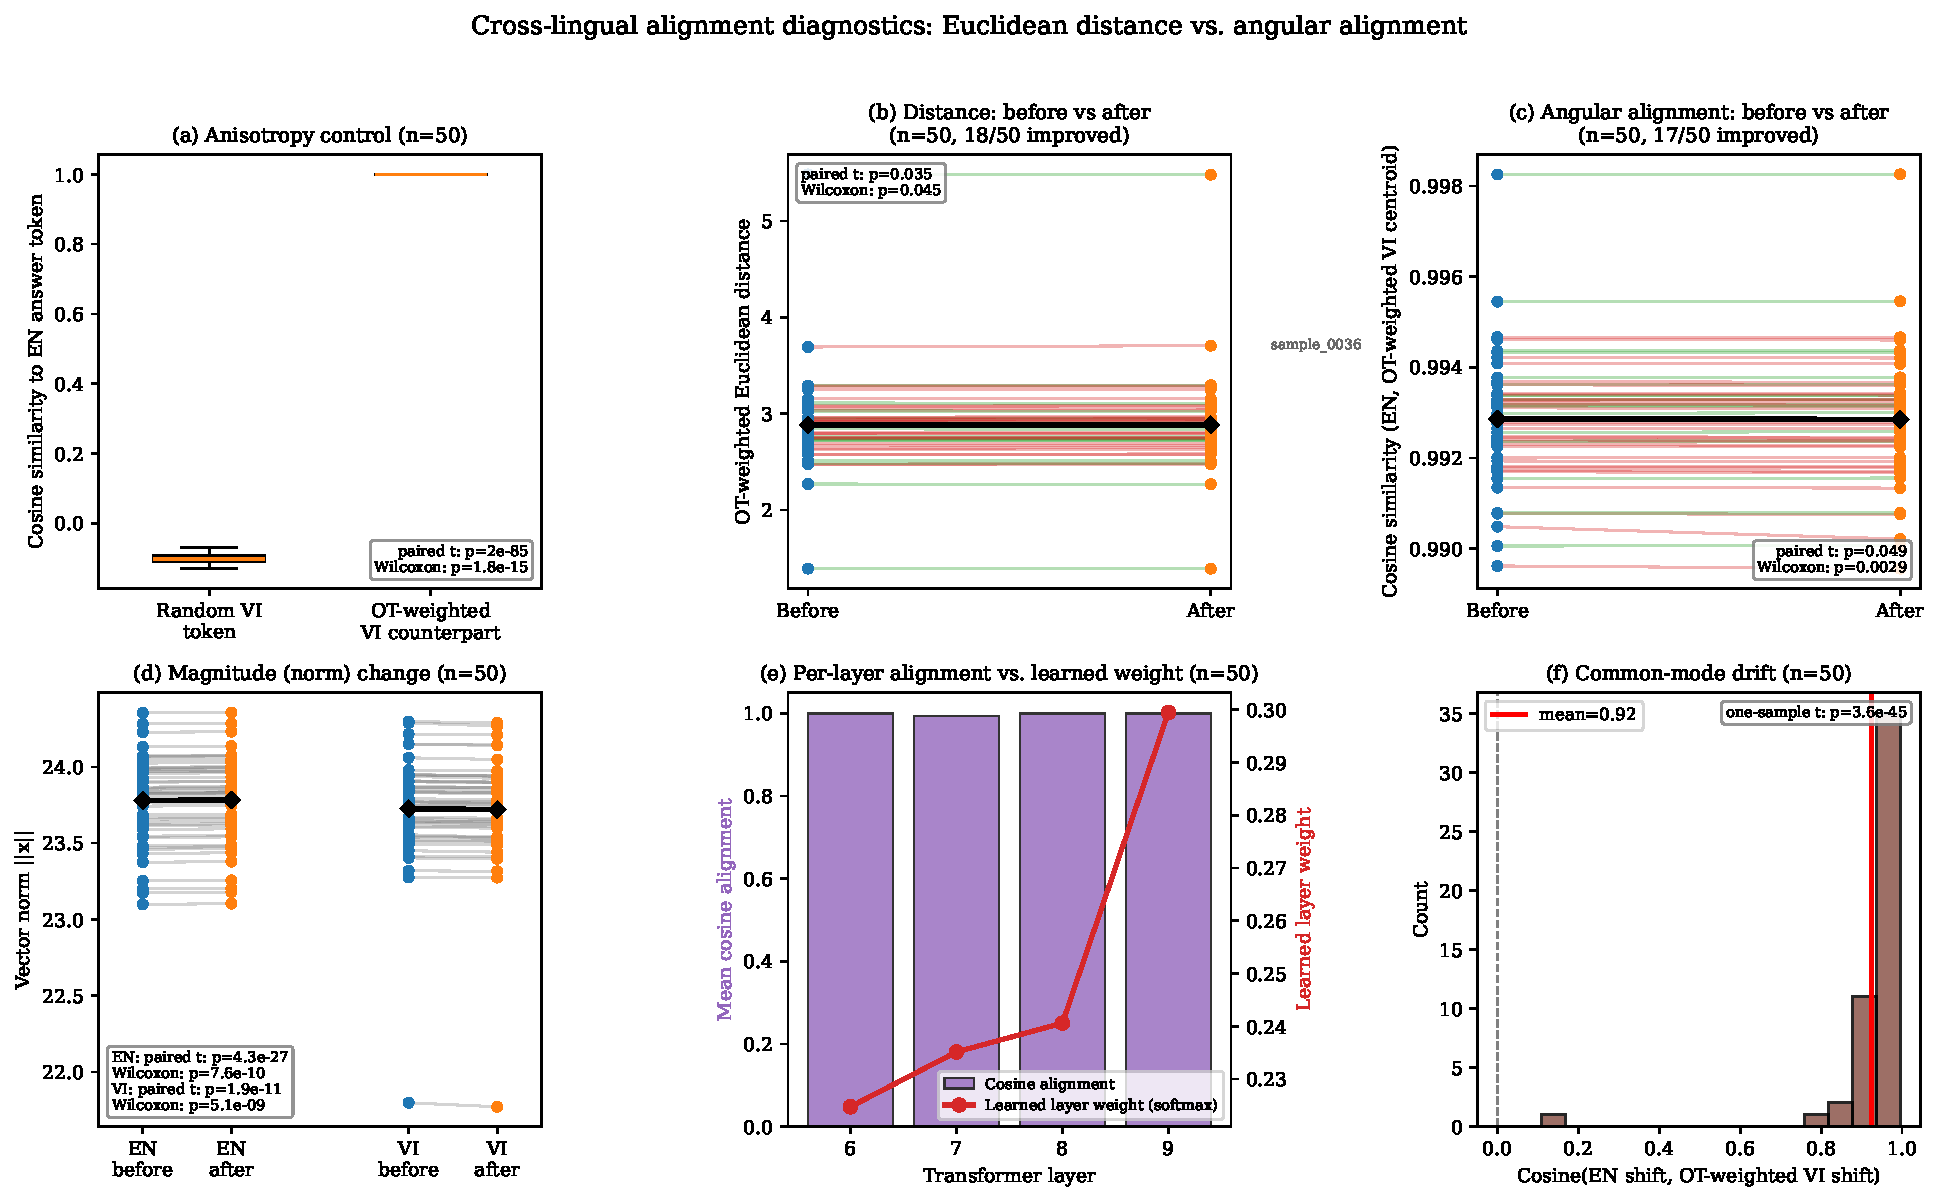
\includegraphics[width=1.05\textwidth]{figures/figure_alignment_summary.pdf}
    \caption{Geometric diagnostics of the OT-weighted cross-lingual alignment ($n=50$ sampled pairs). (a) Anisotropy control: the OT-weighted Vietnamese counterpart is far more similar to the English answer token than a randomly sampled Vietnamese token, ruling out a trivial anisotropy artifact. (b--c) Euclidean distance and angular (cosine) alignment between English and OT-weighted Vietnamese representations, before and after Stage-2 adaptation. (d) Change in representation norm for English and Vietnamese tokens. (e) Per-layer cosine alignment against the learned softmax layer weight (cf.\ Figure~\ref{fig:layer_weights}), showing that the layer receiving the highest learned weight (layer 9) also exhibits the strongest alignment. (f) Common-mode drift: cosine similarity between the English and OT-weighted Vietnamese shift vectors is consistently high (mean $=0.90$), indicating that adaptation moves both representations in a broadly coordinated direction.}
    \label{fig:alignment_diagnostics}
\end{figure*}

Figure~\ref{fig:alignment_diagnostics} summarizes these diagnostics, computed over $n=50$ sampled pairs. Panel (a) confirms that the OT-weighted correspondence is non-trivial: cosine similarity to the true English answer token is near $1.0$ for the OT-selected Vietnamese counterpart, against near-zero for a random Vietnamese token ($p=2.3\times10^{-81}$, paired $t$-test), ruling out a trivial anisotropy artifact.

Panel (b) shows that raw Euclidean distance between English and OT-weighted Vietnamese representations increases slightly but consistently after adaptation: 49 of 50 pairs show an increase, with a median shift of only $+0.005$ and a mean shift of $+0.015$ (paired $t$ $p=0.0023$, Wilcoxon $p=8\times10^{-10}$). Here it is the consistency of direction across nearly all pairs, rather than the magnitude of the shift -- under $1\%$ of the median pre-adaptation distance of $\approx 3.1$ -- that drives significance; a small number of pairs with much larger absolute distances (e.g., sample\_0044) inflate the mean without changing the qualitative pattern.

Panel (c) is more equivocal than panel (b), and we report this honestly rather than the more optimistic picture a smaller sample suggested. At $n=50$, the angular (cosine) alignment shift is \emph{not} statistically significant (paired $t$ $p=0.089$, Wilcoxon $p=0.15$): a bare majority of pairs (33/50) shift in the improving direction, but the median change is essentially zero ($+0.00001$) and the mean is pulled slightly negative by a handful of pairs with larger degradations. An earlier diagnostic on a smaller $n=20$ subset had suggested a clearer positive trend (18/20 improved, Wilcoxon $p=0.012$); this larger and more representative sample does not replicate that effect as statistically reliable, and we treat angular alignment as an open question for this framework rather than a confirmed improvement.

Panel (d) reports the accompanying change in representation norm for both languages ($n=50$), and deserves a direct comment given the role of $\mathcal{L}_{reg}$. Both English and Vietnamese tokens show a statistically significant shift in magnitude (English: paired $t$ $p=3.9\times10^{-76}$, Wilcoxon $p=7.6\times10^{-10}$; Vietnamese: paired $t$ $p=1.5\times10^{-6}$, Wilcoxon $p=2.4\times10^{-6}$), and the English shift is in fact associated with the smaller $p$-value of the two, despite English being the side explicitly anchored by $\mathcal{L}_{reg}$. Computing the underlying effect sizes resolves this: the mean English norm shift is $+0.066$ ($\mathrm{SD}=0.002$, a $0.28\%$ relative change, range $[0.062, 0.070]$ across the 50 pairs), whereas the mean Vietnamese shift is smaller in magnitude ($+0.049$, a $0.21\%$ relative change) but far more variable ($\mathrm{SD}=0.063$, range $[-0.246, 0.078]$). In other words, English does not shift more than Vietnamese in absolute terms -- if anything, slightly less -- but it shifts by an almost identical amount for every sampled pair, which is what drives its more extreme $p$-value under a paired test: statistical significance here reflects the \emph{consistency} of the shift's direction and magnitude across pairs, not its size. This pattern is consistent with the English shift being a small, systematic calibration effect induced uniformly by the LoRA adapters (largely input-independent to first order), rather than input-specific representation drift; the substantially larger and more dispersed Vietnamese shift, in contrast, reflects genuine per-example structural reorganization under the OT-guided pull toward the source space, exactly as the framework is designed to induce. Both shifts remain under $0.3\%$ of the total vector norm, supporting the ``soft anchor, not frozen'' interpretation of $\mathcal{L}_{reg}$ without requiring the encoder to be exactly invariant.

Panel (e) provides direct evidence for the layer-weighting behavior discussed above: alignment quality increases with depth across layers 6--9, mirroring the learned softmax weights. Finally, panel (f) shows that the direction of representation shift induced by adaptation remains highly correlated between languages even at $n=50$ (one-sample $t$-test, $p=7.1\times10^{-33}$, mean cosine $=0.90$), supporting the claim that our coordination mechanism moves source and target representations in a broadly coordinated direction rather than distorting their relative geometry arbitrarily.

\section{Hyperparameter Sensitivity and Loss Scale Normalization}
\label{sec:appendix_sensitivity}
The multi-objective parameters $\lambda_{ot}$, $\lambda_{span}$, and $\lambda_{reg}$ function as fixed loss-scale normalizers, held constant throughout training, to bring different objectives to a comparable magnitude. $\lambda_{margin}$ is the exception: as described in Section~\ref{sec:temporal}, it is time-varying (the $m(\epsilon)$ schedule in Figure~\ref{fig:margin_schedule}), and the value $1.0$ reported in Table~\ref{tab:hyperparameters} refers only to its peak. The domain-consistency coefficient ($\lambda_{reg}$) dominates among the fixed weights with a value of $50.0$, which is structurally required because the native token-level $L_2$ deviation scales within a significantly smaller numerical range ($0.008$ to $0.01$). 

We performed a grid search variation over $\lambda_{reg} \in \{0.0, 10.0, 50.0, 100.0\}$. Setting $\lambda_{reg} < 10.0$ induces a severe representation drift in the shared LoRA blocks, resulting in an immediate collapse of English QA proficiency. Conversely, setting $\lambda_{reg} > 100.0$ over-regularizes the adapter weights, restricting the student's capacity to adjust its latent representations to the target language topology.

\section{Optimization Dynamics: Curriculum vs. Static Margin}
\label{sec:appendix_margin_dynamics}
The full training trajectories comparing the static decision-boundary margin (configuration M5) against our dynamic curriculum margin schedule (configuration M4), along with the accompanying trade-off discussion, are presented in Section~\ref{sec:margin_impact} and Figure~\ref{fig:margin_dynamics_vi_combined} to avoid duplicating the same figures here.

\section{Held-Out English Training Trajectories}
\label{sec:appendix_heldout_curves}
Figures~\ref{fig:margin_dynamics_en_combined} shows the full validation trajectories from a single seed underlying one snapshot of the held-out comparison; Table~\ref{tab:heldout_source} (Section~\ref{sec:margin_impact}) reports the validated multi-seed comparison, where the static schedule (M5) is in fact ahead of the dynamic one (M4) on XQuAD-en by a reliable margin, the reverse of what this single-seed trajectory plot might suggest. We retain the plot here as an illustration of training dynamics rather than as evidence for either configuration's superiority.

\begin{figure}[H]
    \centering
    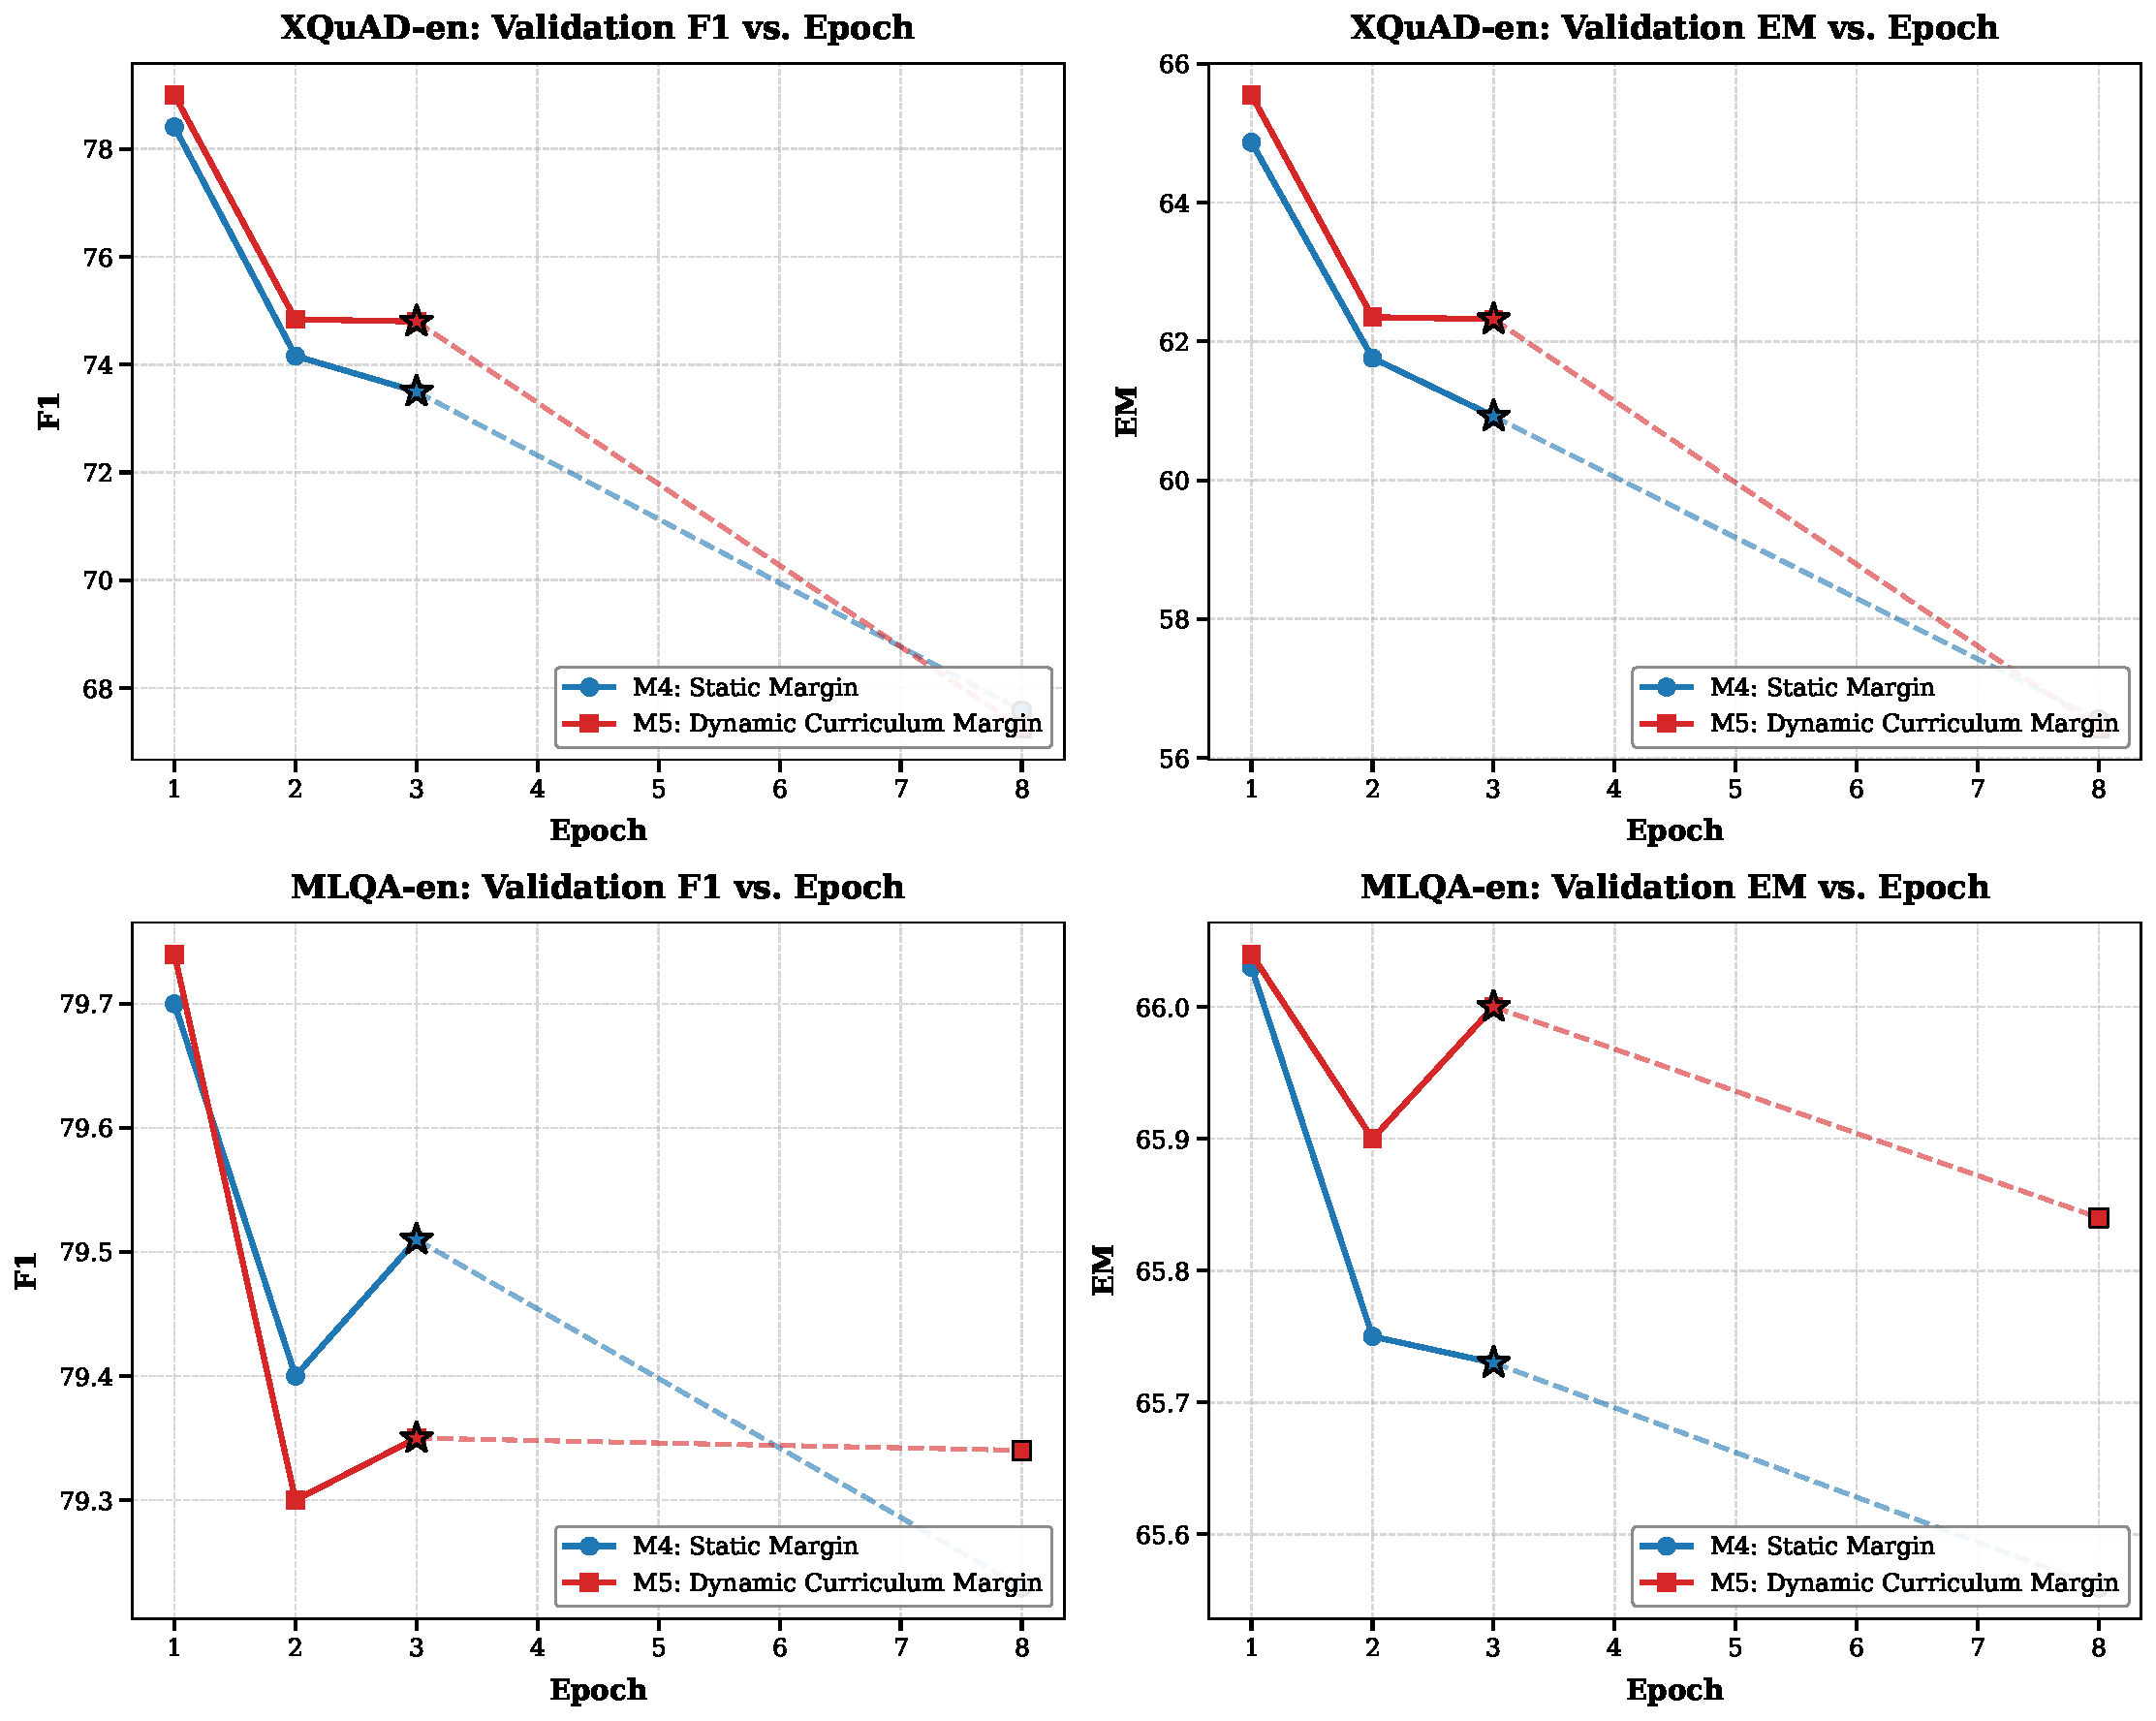
\includegraphics[width=1.05\linewidth]{figures/figure_margin_dynamics_en_combined.pdf}
    \caption{Validation F1 and EM trajectories across 8 training epochs on held-out English XQuAD-en and MLQA-en, comparing the dynamic curriculum schedule (M4) against our static margin constraint (M5).}
    \label{fig:margin_dynamics_en_combined}
\end{figure}

\section{Additional Arabic Ablations: M2 Replication and Static-vs-Dynamic Divergence}
\label{sec:appendix_arabic_margin}
Beyond the M4-vs-M5 comparison, we also ran the M2 (OT-only, global spatial alignment with the domain-consistency anchor active but no span or margin term) configuration on the Arabic branch, to test whether the M2-underperforms-M0 finding central to Section~\ref{sec:ablation_study} (Table~\ref{tab:ablation_study}) replicates on a second, typologically distant language.

\begin{table}[H]
\centering
\small
\begin{tabular}{lcc}
\toprule
\textbf{Benchmark} & \textbf{M0 (Zero-shot)} & \textbf{M2 (OT only)} \\
 & EM~/~F1 & EM~/~F1 \\
\midrule
XQuAD-ar (target) & \textbf{43.53} / \textbf{57.03} & 35.63 / 50.34 \\
MLQA-ar (target) & \textbf{37.26} / \textbf{56.38} & 32.22 / 52.03 \\
\midrule
SQuAD-EN (in-domain) & 64.26 / 72.84 & \textbf{65.67} / \textbf{73.82} \\
XQuAD-en (held-out) & \textbf{63.03} / \textbf{75.75} & 58.49 / 70.96 \\
MLQA-en (held-out) & \textbf{66.51} / \textbf{79.9} & 65.49 / 79.4 \\
\bottomrule
\end{tabular}
\caption{Zero-shot baseline (M0) vs.\ OT-only (M2) on the Arabic branch, at M2's selected checkpoint. Bold marks the better value per metric per row.}
\label{tab:arabic_m2}
\end{table}

The central finding replicates cleanly: on both Arabic target benchmarks, M2 (global OT alignment alone, without span-aware local alignment or margin-based temporal coordination) performs \emph{worse} than the zero-shot baseline M0 -- exactly the pattern observed on Vietnamese (Table~\ref{tab:ablation_study}), confirming that unregulated global OT alignment is not a language-specific failure mode. Interestingly, M2 also slightly \emph{improves} the in-domain SQuAD-EN benchmark over M0 (consistent with the domain-consistency anchor $\mathcal{L}_{reg}$ remaining active in this configuration), while it \emph{degrades} both held-out English benchmarks (XQuAD-en, MLQA-en) relative to M0. This split pattern on the English side -- source in-domain slightly improving while held-out English degrades -- is not something we observed as clearly in the Vietnamese branch and is not something we attempt to explain causally here; we report it as an additional data point for future investigation into how OT-only alignment interacts differently with in-domain versus held-out source-language distributions.

We now turn to the M4-vs-M5 (dynamic vs.\ static margin) comparison on Arabic, using the same selected-checkpoint protocol as Section~\ref{sec:margin_impact}. Table~\ref{tab:arabic_margin} reports the result across both the target-transfer benchmarks (XQuAD-ar, MLQA-ar) and the source-side benchmarks (SQuAD-EN in-domain, XQuAD-en and MLQA-en held-out).

\begin{table}[H]
\centering
\small
\begin{tabular}{lcc}
\toprule
\textbf{Benchmark} & \textbf{M4 (Dynamic)} & \textbf{M5 (Static)} \\
 & EM~/~F1 & EM~/~F1 \\
\midrule
SQuAD-EN (in-domain) & \textbf{65.44} / \textbf{73.81} & 63.77 / 72.57 \\
XQuAD-en (held-out) & 63.85 / 75.82 & \textbf{63.7} / \textbf{76.81} \\
MLQA-en (held-out) & \textbf{66.46} / \textbf{79.92} & 66.21 / 79.52 \\
\midrule
XQuAD-ar (target) & 46.3 / 64.7 & \textbf{47.31} / \textbf{65.26} \\
MLQA-ar (target) & 37.25 / \textbf{56.64} & \textbf{37.59} / 56.5 \\
\bottomrule
\end{tabular}
\caption{Dynamic (M4) vs.\ static (M5) margin schedule on the Arabic branch, at each configuration's selected checkpoint. Bold marks the better value per metric per row; near-ties (within 0.15 points) are not bolded on either side.}
\label{tab:arabic_margin}
\end{table}

Unlike the single-seed snapshot originally reported for Vietnamese, the validated multi-seed pattern (Table~\ref{tab:heldout_source}) shows static (M5) ahead on Vietnamese target benchmarks, and the Arabic results here are, if anything, a partial mirror rather than a contradiction: on the in-domain SQuAD-EN benchmark, the dynamic schedule (M4) is \emph{better} than the static one on both metrics, while on the Arabic target benchmarks, the static schedule (M5) is better on XQuAD-ar on both metrics and on MLQA-ar EM, with M4 only marginally ahead on MLQA-ar F1. Only on the held-out MLQA-en benchmark does a clear direction (M4 ahead) hold for Arabic; XQuAD-en is a near-tie for Arabic (63.85 vs.\ 63.7 EM, within noise) with M5 ahead on F1. Taken together with Section~\ref{sec:margin_impact}'s Vietnamese multi-seed result, the overall picture across both languages is one of no consistent, reliable direction of preference between static and dynamic scheduling -- reinforcing rather than complicating the paper's central methodological conclusion.

We do not attempt to force these Arabic results into the same causal narrative developed for Vietnamese in Section~\ref{sec:margin_impact}. Instead, we read this as evidence that the specific trade-off between static and dynamic margin scheduling is not a fixed, language-independent property of the framework, but interacts with language-specific factors (e.g., tokenization granularity, morphological distance from English, or the size and quality of the Arabic parallel training corpus). This directly supports the caution already raised in our Limitations section against assuming the Vietnamese-specific numerical trade-offs generalize unchanged to typologically distant languages, and suggests that the choice between static and dynamic margin scheduling may need to be validated per target language rather than fixed a priori.

\section{Qualitative Case Study: Visualizing Answer Span Boundaries}
\label{sec:appendix_case_study}
To qualitatively demonstrate how our coordinated framework prevents answer-boundary ambiguity, we extract a translation-shifted paragraph sample from the evaluation benchmark. 
\begin{figure}[H]
    \centering
    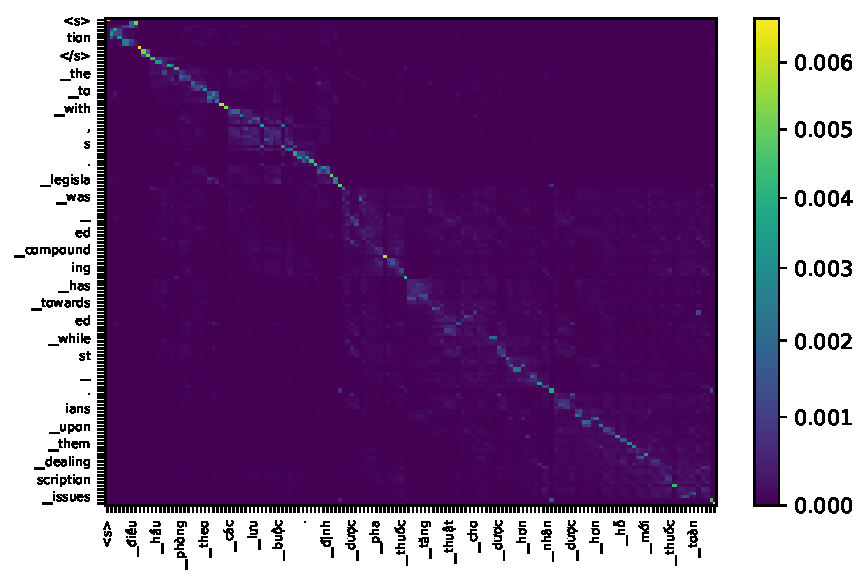
\includegraphics[width=1.05\linewidth]{figures/figure2_ot_heatmap.pdf}
    \caption{Visualization of the log-domain Sinkhorn transport plan ($\gamma$) aligning source English tokens (rows) with target Vietnamese tokens (columns) for a representative XQuAD-vi example. Transport mass concentrates near the diagonal with a few coherent off-diagonal bands, indicating that the plan recovers meaningful token-level correspondence despite word-segmentation and word-order differences between the two languages.}
    \label{fig:case_study}
\end{figure}

The transport plan visualization in Figure \ref{fig:case_study} shows that alignment mass is concentrated in coherent, low-noise bands rather than being diffusely spread across unrelated tokens, consistent with our claim that the OT plan produces a structurally meaningful cross-lingual correspondence. This qualitative pattern is consistent with the quantitative margin behavior in Table~\ref{tab:ablation_study}: because the Curriculum Margin keeps the top-1/top-2 task-space logit gap discriminative throughout training, the resulting transport-guided pseudo-labels translate into coherent rather than diffuse predicted spans. A side-by-side visualization of predicted spans under the static versus dynamic margin schedule on this same example is left for future work.
\end{document}